% -*- Mode:TeX -*-

%% IMPORTANT: The official thesis specifications are available at:
%%            http://libraries.mit.edu/archives/thesis-specs/
%%
%%            Please verify your thesis' formatting and copyright
%%            assignment before submission. If you notice any
%%            discrepancies between these templates and the 
%%            MIT Libraries' specs, please let us know
%%            by e-mailing thesis@mit.edu

%% The documentclass options along with the pagestyle can be used to generate
%% a technical report, a draft copy, or a regular thesis. You may need to
%% re-specify the pagestyle after you \include cover.tex. For more
%% information, see the first few lines of mitthesis.cls. 

%\documentclass[12pt,vi,twoside]{mitthesis}
%%
%%  If you want your thesis copyright to you instead of MIT, use the
%%  ``vi'' option, as above.
%%
%\documentclass[12pt,twoside,leftblank]{mitthesis}
%%
%% If you want blank pages before new chapters to be labelled ``This
%% Page Intentionally Left Blank'', use the ``leftblank'' option, as
%% above. 

\documentclass[12pt,oneside]{report}
\usepackage{lgrind}
\usepackage{subfiles}
%% These have been added at the request of the MIT Libraries, because
%% some PDF conversions mess up the ligatures.  -LB, 1/22/2014
\usepackage{cmap}
\usepackage[T1]{fontenc}
\pagestyle{plain}

%% This bit allows you to either specify only the files which you wish to
%% process, or `all' to process all files which you \include.
%% Krishna Sethuraman (1990).

%\typein [\files]{Enter file names to process, (chap1,chap2 ...), or `all' to process all files:}
\def\all{all}
\ifx\files\all \typeout{Including all files.} \else %\typeout{Including only \files.} \includeonly{\files} \fi

\begin{document}

% -*-latex-*-
% 
% For questions, comments, concerns or complaints:
% thesis@mit.edu
% 
%
% $Log: cover.tex,v $
% Revision 1.9  2019/08/06 14:18:15  cmalin
% Replaced sample content with non-specific text.
%
% Revision 1.8  2008/05/13 15:02:15  jdreed
% Degree month is June, not May.  Added note about prevdegrees.
% Arthur Smith's title updated
%
% Revision 1.7  2001/02/08 18:53:16  boojum
% changed some \newpages to \cleardoublepages
%
% Revision 1.6  1999/10/21 14:49:31  boojum
% changed comment referring to documentstyle
%
% Revision 1.5  1999/10/21 14:39:04  boojum
% *** empty log message ***
%
% Revision 1.4  1997/04/18  17:54:10  othomas
% added page numbers on abstract and cover, and made 1 abstract
% page the default rather than 2.  (anne hunter tells me this
% is the new institute standard.)
%
% Revision 1.4  1997/04/18  17:54:10  othomas
% added page numbers on abstract and cover, and made 1 abstract
% page the default rather than 2.  (anne hunter tells me this
% is the new institute standard.)
%
% Revision 1.3  93/05/17  17:06:29  starflt
% Added acknowledgements section (suggested by tompalka)
% 
% Revision 1.2  92/04/22  13:13:13  epeisach
% Fixes for 1991 course 6 requirements
% Phrase "and to grant others the right to do so" has been added to 
% permission clause
% Second copy of abstract is not counted as separate pages so numbering works
% out
% 
% Revision 1.1  92/04/22  13:08:20  epeisach

% NOTE:
% These templates make an effort to conform to the MIT Thesis specifications,
% however the specifications can change. We recommend that you verify the
% layout of your title page with your thesis advisor and/or the MIT 
% Libraries before printing your final copy.

\title{Fault-Tolerant All-Pairs Mincuts}

\author{Abhyuday Pandey\\(BT/CSE/170039)\\\\\\\textbf{Supervisor:} Dr. Surender Baswana}
\date{\today}

% \maketitle
% \begin{center}
%     
\includegraphics[]{templates/iitk_logo.jpg}
% \end{center}

\makeatletter
    \begin{titlepage}
        \begin{center}
            {\huge \bfseries  \@title }\\[4ex] 
            {\large  Abhyuday Pandey}\\[4ex]
            {\large BT/CSE/170039}\\[4ex]
            {\large \textbf{Supervisor:} Dr. Surender Baswana}\\[20ex]
            
\includegraphics[height=5cm]{templates/iitk_logo.jpg}\\[20ex] 
            
            {\large \@date}
        \end{center}
    \end{titlepage}
\makeatother
\thispagestyle{empty}
\newpage

% The abstractpage environment sets up everything on the page except
% the text itself.  The title and other header material are put at the
% top of the page, and the supervisors are listed at the bottom.  A
% new page is begun both before and after.  Of course, an abstract may
% be more than one page itself.  If you need more control over the
% format of the page, you can use the abstract environment, which puts
% the word "Abstract" at the beginning and single spaces its text.

%% You can either \input (*not* \include) your abstract file, or you can put
%% the text of the abstract directly between the \begin{abstractpage} and
%% \end{abstractpage} commands.

% First copy: start a new page, and save the page number.
% Uncomment the next line if you do NOT want a page number on your
% abstract and acknowledgments pages.
% \pagestyle{empty}
\section*{Abstract}
\subfile{abstract}
\vfill
% {These results are submitted to the $53^{rd}$ Annual ACM Symposium on Theory of Computing
% June $21-25, 2021$ in Rome, Italy.}

\pagebreak
% Additional copy: start a new page, and reset the page number.  This way,
% the second copy of the abstract is not counted as separate pages.
% Uncomment the next 6 lines if you need two copies of the abstract
% page.
% \setcounter{page}{\thesavepage}
% \begin{abstractpage}
% % $Log: abstract.tex,v $
% Revision 1.1  93/05/14  14:56:25  starflt
% Initial revision
% 
% Revision 1.1  90/05/04  10:41:01  lwvanels
% Initial revision
% 
%
%% The text of your abstract and nothing else (other than comments) goes here.
%% It will be single-spaced and the rest of the text that is supposed to go on
%% the abstract page will be generated by the abstractpage environment.  This
%% file should be \input (not \include 'd) from cover.tex.

Let $G=(V,E)$ be an undirected unweighted graph on $n$ vertices and $m$ edges. We address the problem of sensitivity oracle for all-pairs mincuts in $G$ defined as follows.

Build a compact data structure that, on receiving a pair of vertices $s,t\in V$ and insertion/deletion of any edge as query, can efficiently report the value of the mincut between $s$ and $t$ upon the update.

To the best of our knowledge, there exists no data structure for this problem which takes $o(mn)$ space and a non-trivial query time. Recently, Baswana, Gupta, and Knollman \cite{DBLP:conf/esa/BaswanaGK20} gave a data structure that can handle single edge insertion in ${\cal O}(n^2)$ space and ${\cal O}(1)$ query time. We present the following results.

\begin{enumerate}
    \item We present a sensitivity oracle for all-pairs mincuts. Our data structure guarantees ${\cal O}(1)$ query time. The space occupied by this data structure is ${\cal O}(n^2)$ which matches the worst-case size of a graph on $n$ vertices. A resulting $(s,t)$-mincut after edge insertion/deletion can be reported in ${\cal O}(n)$ time which is optimal. Our data structure also subsumes the results of Baswana, Gupta, and Knollman \cite{DBLP:conf/esa/BaswanaGK20}.
    \item We give conditional lower bounds on data structures that can handle dual-deletions (or dual-faults) for a $(s,t)$-mincut. We also give a conditional lower bound on a data structure storing all static $(\{s,u\},\{t,v\})$-mincut values with fixed $s,t \in V$. This implies a conditional lower bound for a generalized flow tree for $2 \times 2$ mincuts, i.e. a data structure that can report the value of static $(\{s,u\},\{t,v\})$-mincut for given vertices $s,t,u,v \in V$.
\end{enumerate}

Some parts of this work have been taken from a recent research of Baswana and Pandey \cite{DBLP:journals/corr/BaswanaP20}, but presented here for sake of continuity. 

% \end{abstractpage}

\section*{Acknowledgments}

I am deeply indebted to Prof Surender Baswana for allowing me to work with him. I am thankful to him for having regular meetings despite his busy schedule and helping me acquire the necessary perseverance for solving a research problem. I would like to thank Prof Yefim Dinitz and Prof Alek Vainshtein for their seminal work ``The connectivity carcass of a vertex subset in a graph and its incremental maintenance" which appeared in STOC 1994 and subsequently in SIAM Journal of Computing 2000 edition. The paper truly captures the entire anatomy of mincuts and also forms the foundation of our results. Last but not the least, I would like to thank my parents and sister for their incredible and unconditional support in this pandemic. 
%%%%%%%%%%%%%%%%%%%%%%%%%%%%%%%%%%%%%%%%%%%%%%%%%%%%%%%%%%%%%%%%%%%%%%
% -*-latex-*-

% Some departments (e.g. 5) require an additional signature page.  See
% signature.tex for more information and uncomment the following line if
% applicable.
% \include{signature}
\pagestyle{plain}
  % -*- Mode:TeX -*-
%% This file simply contains the commands that actually generate the table of
%% contents and lists of figures and tables.  You can omit any or all of
%% these files by simply taking out the appropriate command.  For more
%% information on these files, see appendix C.3.3 of the LaTeX manual. 
\tableofcontents
% \newpage
% \listoffigures
% \newpage
% \listoftables


%% This is an example first chapter.  You should put chapter/appendix that you
%% write into a separate file, and add a line \include{yourfilename} to
%% main.tex, where `yourfilename.tex' is the name of the chapter/appendix file.
%% You can process specific files by typing their names in at the 
%% \files=
%% prompt when you run the file main.tex through LaTeX.
\chapter{Introduction}

Graph mincut is a fundamental structure in graph theory with numerous applications. Let $G=(V,E)$ be an undirected unweighted connected graph on $n=|V|$ vertices and $m=|E|$ edges.
Two most common types of mincuts are global mincuts and pairwise mincuts. A set of edges with the least cardinality whose removal disconnects the graph is called a global mincut. For any pair of vertices $s,t\in V$, 
a set of edges with the least cardinality whose removal disconnects $t$ from $s$ is called a pairwise mincut for $s,t$ or simply a $(s,t)$-mincut. A more general notion is that of Steiner mincuts. For any given set $S\subseteq V$ of vertices, a set of edges with the least cardinality whose removal disconnects $S$ is called a Steiner mincut for $S$. It is easy to observe that the Steiner mincuts for $S=V$ are the global mincuts and for $S=\{s,t\}$ are $(s,t)$-mincuts.

While designing an algorithm for a graph problem, one usually assumes that the underlying graph is static. But, this assumption is unrealistic for most of the real-world graphs where vertices and/or edges do undergo change, though occasionally. Sensitivity Oracles can be used to efficiently make a query for a single update/delete operation. The data structure can be preprocessed offline.

% In the past, many elegant fault-tolerant algorithms have been designed for various classical problems, namely,  connectivity \cite{DBLP:conf/stoc/Chan02,DBLP:journals/algorithmica/FrigioniI00,DBLP:journals/siamcomp/ChanPR11,DBLP:conf/soda/DuanP17}, shortest-paths \cite{DBLP:conf/stoc/BernsteinK09,DBLP:journals/siamcomp/DemetrescuTCR08,DBLP:conf/stoc/ChechikC20}, graph spanners \cite{ChechikLPR10,DBLP:journals/tcs/BraunschvigCPS15}, SCC \cite{DBLP:journals/algorithmica/BaswanaCR19} , DFS tree \cite{DBLP:journals/siamcomp/BaswanaCC019}, and BFS structure \cite{DBLP:journals/talg/ParterP16,DBLP:journals/talg/ParterP18}. However, little is known about fault-tolerant data structures for various types of mincuts. The problem of fault-tolerant all-pairs mincuts aims at preprocessing a given graph to build a compact data structure so that the following query can be answered efficiently for any $s,t\in V$ and $(x,y)\in E$.\\

% \noindent
% FT-mincut$(u,v,x,y)$: Report the value of $(u,v)$-mincut in $G$ after the failure/removal of edge $(x,y)$, if exists, from $E$.\\

% \noindent
% % {\textsc{ft-mincut}}$(s,t,x,y)$: Report a $(s,t)$-mincut in $G$ after the failure of edge $(x,y)$, if exists, from $E$.\\
% {\textsc{ft-mincut}}$(s,t,x,y)$: Report a $(s,t)$-mincut in $G$ after the failure of edge $(x,y)$.\\



\section{Previous Results} 


There exists a classical ${\cal O}(n)$ size data structure that stores all-pairs mincuts \cite{GH61} known as Gomory-Hu tree. It is a tree on the vertex set $V$ that compactly stores a mincut between each pair of vertices. However, we cannot determine using a Gomory-Hu tree whether the failure of an edge will affect the $(s,t)$-mincut unless this edge belongs to the $(s,t)$-mincut present in the tree. We can get a fault-tolerant data structure by storing $m$ Gomory-Hu trees, one for each edge failure. The overall data structure occupies ${\cal O}(mn)$ space and takes ${\cal O}(1)$ time to report the value of $(s,t)$-mincut for any $s,t\in V$ upon failure of a given edge. A new $(s,t)$-mincut can itself be reported in ${\cal O}(n)$ time. 


For handling edge insertions, Baswana, Gupta and Knollman \cite{DBLP:conf/esa/BaswanaGK20} recently gave a data structure that can report the value of a $(s,t)$-mincut upon insertion of an edge. Moreover, a $(s,t)$-mincut incorporating the change can be reported in ${\cal O}(n)$ time.


Combining the above two results, a sensitivity oracle can be obtained that uses ${\cal O}(mn)$ space. However, the ${\cal O}(mn)$ space occupied by this data structure is far from the size of the graph. To the best of our knowledge, there exists no data structure for this problem which takes $o(mn)$ space and a non-trivial query time.



\section{Our Contribution} We present a space efficient sensitivity oracle for the all-pairs mincuts problem in an undirected unweighted multigraph. The data structure occupies ${\cal O}(n^2)$ space while achieving the optimal ${\cal O}(1)$ query time to report the value of $(s,t)$-mincut for any $s,t\in V$ upon deletion/insertion of any given edge. A resulting $(s,t)$-mincut incorporating the change can be reported in ${\cal O}(n)$ time.

In order to design our data structure, we present an efficient solution for a related problem of independent interest, called edge-containment query on a mincut defined as follows.\\

\noindent
{\textsc{edge-contained}}$(s,t,(x,y))$: Check if a given edge $(x,y)\in E$ belong to some $(s,t)$-mincut.\\

Using a data structure for this problem, we can answer a deletion query upon failure of edge $(x,y)$ by performing the corresponding edge-containment query. The value of $(s,t)$-mincut will reduce by unity if the edge-containment query evaluates to true. We can keep a Gomory-Hu tree of ${\cal O}(n)$ size as an auxiliary data structure to lookup the old value of $c_{s,t}$. The following fact allows us to do so.

\begin{fact}
\label{fact:(x,y)-lies-in-(s,t)-mincut}
The value of $(s,t)$-mincut decreases on deletion of an edge $(x,y)$ if and only if $(x,y)$ lies in \textit{some} $(s,t)$-mincut.
\end{fact}


We give conditional lower bounds for the following problems.

\begin{enumerate}
    \item Data structures that can handle dual-deletions (or dual-faults) for a $(s,t)$-mincut. In particular, we show that a data structure that can handle deletion (or failure) of two edges for a $(s,t)$-mincut even for fixed pair of vertices $s,t\in V$ requires ${\tilde \Omega}(n^2)$ space for non-trivial query time.
    \item Generalized flow tree for $2 \times 2$ mincuts, i.e. a data structure that can report the value of static $(\{s,u\},\{v,t\})$-mincut for given vertices $s,t,u,v \in V$. We show that even if we fix $s,t \in V$, the data structure must require ${\tilde \Omega}(n^2)$ space for non-trivial query time.
\end{enumerate}


\section{Related Work} 
A related problem is that of maintaining mincuts in a dynamic environment. Until recently, most of the work on this problem has been limited to global mincuts. Thorup \cite{DBLP:journals/combinatorica/Thorup07} gave a Monte-Carlo algorithm for maintaining a global mincut of polylogarithmic size with ${\tilde {\cal O}}(\sqrt{n})$ update time.  He also showed how to maintain a global mincut of arbitrary size with $1+o(1)$-approximation within the same time-bound. Goranci, Henzinger and Thorup \cite{DBLP:journals/talg/GoranciHT18} gave a deterministic incremental algorithm for maintaining a global mincut with amortized ${\tilde{\cal O}}(1)$ update time and ${\cal O}(1)$ query time. Hartmann and Wagner \cite{DBLP:conf/isaac/HartmannW12} designed a fully dynamic algorithm for maintaining all-pairs mincuts  which provided significant speedup in many real-world graphs, however, its worst-case asymptotic time complexity is not better than the best static algorithm for an all-pairs mincut tree. Recently, there is a fully-dynamic algorithm \cite{DBLP:journals/corr/abs-2005-02368} that approximates all-pairs mincuts up to a nearly logarithmic factor in ${\tilde{\cal O}}(n^{2/3} )$ amortized time against an oblivious adversary, and ${\tilde{\cal O}}(m^{3/4} )$ time against an adaptive adversary. To the best of our knowledge, there exists no non-trivial dynamic algorithm for all-pairs \textit{exact} mincut. We feel that our insights in this paper may be helpful in this problem.

\noindent


% \section{Overview of our results} 

% Dinitz and Vainshtein \cite{DBLP:journals/siamcomp/DinitzV00}
% presented a novel data structure called {\em connectivity carcass} that stores all Steiner mincuts for a given Steiner set $S\subseteq V$ in ${\cal O}(\min(m,nc_S))$ space, where $c_S$ is the value of Steiner mincut. %We observe that this data structure can be used easily to design a fault-tolerant data structure for all-pairs mincuts that occupies $O(mn)$-space. 
% Katz, Katz, Korman and Peleg \cite{DBLP:journals/siamcomp/KatzKKP04} presented a data structure of ${\cal O}(n)$ size for labeling scheme of all-pairs mincuts. This structure hierarchically partitions the vertices based on their connectivity in the form of a rooted tree. In this tree, each leaf node is a vertex in set $V$ and each internal node $\nu$ stores the Steiner mincut value of the set $S(\nu)$ of leaf nodes in the subtree rooted at $\nu$. %stores all-pairs mincut value.
% % Apparently, both these data structures seem to be designed for a static graph. 
% We observe that if each internal node $\nu$ of the hierarchy tree
% is augmented with the connectivity carcass of $S(\nu)$, we get a data structure for the edge-containment query. This data structure occupies ${\cal O}(mn)$ space. An edge-containment query can be answered using the connectivity carcass at the Lowest Common Ancestor (LCA) of the given pair of vertices.
% %following, more generic, fault-tolerant query :

% As we move down the hierarchy tree, the size of Steiner set associated with the internal node reduces. So, to make the data structure more compact, a possible approach is to associate a smaller graph $G_\nu$ for each internal node $\nu$ that is {\em small enough} to improve the overall space-bound, yet {\em large enough} to retain the internal connectivity of set $S(\nu)$. 
% However, such a compact graph cannot directly answer the edge-containment query as it does not even contain the information about all edges in $G$. A possible way to overcome this challenge is to transform any edge-containment query in graph $G$ to an equivalent query in graph $G_{\nu}$. In this paper, we show that not only such a transformation exists, but it can also be computed efficiently. We model the query transformation as a multi-step procedure. The following result captures a single step of this procedure.

% % The key observation that allows us to do query transformation is as follows. 
% Given an undirected graph $G=(V,E)$ and a Steiner set $S\subseteq V$, let $S'\subset S$ be any maximal set with connectivity strictly greater than that of $S$. We can build a quotient graph $G_{S'}=(V_{S'},E_{S'})$ such that $S' \subset V_{S'}$ with the following property.

% {\em
% For any two vertices $s,t \in S'$ and any set of edges $E_y$ incident on vertex $y$ in $G$, there exists a set of edges $E_{y'}$ incident on a vertex $y'$ in $G_{S'}$ such that $E_y$ lies in a $(s,t)$-mincut in $G$ if and only if $E_{y'}$ lies in a $(s,t)$-mincut in $G_{S'}$. 
% }

% We build graph $G_\mu$ associated with each internal node $\mu$ of the hierarchy tree as follows. For the root node $r$, $G_r = G$. For any other internal node $\mu$, we use the above result to build the graph $G_{\mu}$ from $G_{\mu'}$, where $\mu'$ is the parent of $\mu$. 
% Our data-structure is the hierarchy tree where each internal node $\mu$ is augmented with the connectivity carcass for $G_\mu$ and the Steiner set $S(\mu)$. A high-level description of our query algorithm is as follows. 
% % We move from the root node to the LCA of $s$ and $t$.
% We traverse the path from the root node to the LCA of $s$ and $t$.
% % We keep transforming an edge-containment query for each edge in this path. 
% We keep transforming the edge-containment query for each edge in this path.
% At the LCA of $s$ and $t$, we stop and perform the query using the connectivity carcass 
% % augmented at this node
% stored at this node.
% Following a rigorous analysis, we show that this data structure takes only ${\cal O}(m)$ space and can answer any edge-containment query in ${\cal O}(\min(m,nc_{s,t}))$ time.

% \section{Organization of the paper:}

% In addition to the basic notations, Section \ref{sec:prelimiaries} presents compact representation for various mincuts. Section \ref{sec:query-transformation} gives insights into $3$-vertex mincuts that form the foundation for transforming an edge-containment query in original graph to a compact graph. We give the construction of compact graph for query transformation in Section \ref{sec:compact-graph-section}.
% Using this compact graph as a building block, we present the data structures for edge-containment query in Section \ref{sec:final-ds}.
\chapter{Preliminaries}


%\subsection{Notations and lemmas on mincuts}
Let $G=(V,E)$ be an undirected unweighted multigraph without self-loops. To contract (or compress) a set of vertices $U\subseteq V$ means to replace all vertices in $U$ by a single vertex $u$, delete all edges with both endpoints in $u$ and for every edge which has one endpoint in $U$, replace this endpoint by $u$. A graph obtained by performing a sequence of vertex contractions is called a {\em quotient} graph of $G$.


For any given $A,B\subset V$ such that $A\cap B=\emptyset$, we use $c(A,B)$ to denote the number of edges with one endpoint in $A$
and another in $B$. Overloading the notation, we shall use $c(A)$ for $c(A,\bar{A})$.

\begin{definition}[$(s,t)$-cut]
A subset of edges whose removal disconnects $t$ from $s$ is called an $(s,t)$-cut. An $(s,t)$-mincut is an $(s,t)$-cut of minimum cardinality. 
\label{def:(u,v)-cut}
\end{definition}

\begin{definition}[set of vertices defining a cut]
A subset $A\subset V$ is said to define an ($s,t$)-cut if $s\in A$ and $t\notin A$. The corresponding cut is denoted by cut$(A,\bar{A})$ or more compactly cut$(A)$.  
\label{def:set-definiting-a-cut}
\end{definition}

The following lemma exploits the undirectedness of the graph.
\begin{lemma}
Let $x,y,z$ be any three vertices in $G$. If $c_{x,y}>c$ and $c_{y,z}>c$, then $c_{x,z}>c$ as well. 
\label{lem:triangle-inequality}
\end{lemma}

When there is no scope of confusion, we do not distinguish between a mincut and the set of vertices defining the mincut. 
We now state a well-known property of cuts.
% \begin{lemma}[Submodularity of cuts]
% For any two subsets $A,B\subset V$, the following inequality holds.
% \[ c(A) +c(B) \ge c(A\cup B) + c(A\cap B) \]
% \label{lem:submodularity}
% \end{lemma}
\begin{lemma}[Submodularity of cuts]
For any two subsets $A,B\subset V$, ~
$ c(A) +c(B) \ge c(A\cup B) + c(A\cap B)$.
\label{lem:submodularity}
\end{lemma}


%The proof of the following lemma exploits just the property of a $(u,v)$-mincut.
\begin{lemma}
Let $S \subset V$ define an $(s,t)$-mincut with $s\in S$. For any subset $S'\subset V\setminus S$ with $v\notin S'$,
\[ 
c(S,S') \le c(S,V\setminus (S\cup S'))
\]
\label{lem:subset-property-of-min-cut}
\end{lemma}
\vspace{-10mm}
\section{Compact representation for all \texorpdfstring{$(s,t)$}{(s,t)}-mincuts}
Dinitz and Vainshtein \cite{DBLP:journals/siamcomp/DinitzV00} showed that there exists a quotient graph of $G$ that compactly stores all $(s,t)$-mincuts. This graph is called strip ${\cal D}_{s,t}$. The 2 node to which $s$ and $t$ are mapped in ${\cal D}_{s,t}$ are called the terminal nodes, denoted by ${\bf s}$ and ${\bf t}$ respectively. Every other node is called a non-terminal node. We now elaborate some interesting properties of the strip ${\cal D}_{s,t}$.
% by Dinitz and Vainshtein \cite{DBLP:journals/siamcomp/DinitzV00}

 Consider any non-terminal node $v$, and let $E_v$ be the set of edges incident on it in ${\cal D}_{s,t}$. There exists a unique partition, called {\em inherent partition}, of $E_v$ into 2 subsets of equal sizes. These subsets are called the 2 sides of the inherent partition of $E_v$. 
 %Dinitz and Vainshtein established the following very interesting property of this inherent partition.
 Interestingly, if we traverse ${\cal D}_{s,t}$ such that upon visiting any non-terminal node using an edge from one side of its inherent partition, the edge that we traverse while leaving it belong to the other side of the inherent partition, then no node will be visited again. Such a path is called a {\em coherent} path in ${\cal D}_{s,t}$. Furthermore, if we begin traversal from a non-terminal node $u$ along one side of its inherent partition and keep following a coherent path we are bound to reach the terminal ${\bf s}$ or terminal ${\bf t}$. So the two sides of the inherent partitions can be called side-${\bf s}$
 and side-${\bf t}$ respectively.
It is because of these properties
that the strip ${\cal D}_{s,t}$ can be viewed as an undirected analogue of a directed acyclic graph with a single source and a single sink. 

A cut in the strip ${\cal D}_{s,t}$ is said to be a \textit{transversal} if each coherent path in ${\cal D}_{s,t}$ intersects it at most once. The following lemma provides the key insight for representing all $(s,t)$-mincuts through the strip ${\cal D}_{s,t}$.
\begin{lemma}[\cite{DBLP:journals/siamcomp/DinitzV00}]
    $A\subset V$ defines a $(s,t)$-mincut if and only if $A$ is a transversal in ${\cal D}_{s,t}$.
    \label{lem:mincut-transversal}
\end{lemma}

We now state the following two lemmas that can be viewed as a corollary of Lemma \ref{lem:mincut-transversal}.

\begin{lemma}
A $(s,t)$-mincut contains a set of edges $E_y$ incident on vertex $y$ if and only if all edges in $E_y$ must belong to the same side of the inherent partition of the node containing $y$ in strip ${\cal D}_{s,t}$.
\label{lem:E_y-edges-same-side}
\end{lemma}

\begin{lemma} 
If $A\subset V$ defines a $(s,t)$-mincut with $s\in A$, then $A$ can be merged with the terminal node ${\mathbf s}$ in ${\cal D}_{s,t}$ to get the strip ${\cal D}_{A,t}$ that stores all those $(s,t)$-mincuts that enclose $A$.
\label{lem:strip-A}
\end{lemma}


Consider any non-terminal node $x$. Let ${\cal R}_s(x)$ be the set of all the nodes $y$ in ${\cal D}_{s,t}$ that are reachable from $x$ through coherent paths that originate from the side-${\bf s}$ of the inherent partition of $x$ -- notice that all these paths will terminate at ${\bf s}$. 
It follows from the construction that ${\cal R}_s(x)$ defines a transversal in
${\cal D}_{s,t}$. We call ${\cal R}_s(x)$ the \textit{reachability cone} of $x$ towards $s$. 
The $(s,t)$-mincut defined by ${\cal R}_s(x)$ is the nearest mincut from $\{s,x\}$ to $t$. 
Interestingly, each transversal in ${\cal D}_{s,t}$, and hence each $(s,t)$-mincut, is a union of the reachability cones of a subset of nodes of ${\cal D}_{s,t}$ in the direction of $s$. We now state the following Lemma that we shall crucially use.

\begin{lemma}[\cite{DBLP:journals/siamcomp/DinitzV00}]
If $x_1,\ldots, x_k$ are any non-terminal nodes in strip ${\cal D}_{s,t}$,  the union of the reachability cones of $x_i$'s in the direction of ${\mathbf s}$ defines the nearest mincut between $\{s, x_1,\ldots, x_k\}$ and $t$.
\label{lem:reachability-cones}
\end{lemma} 


\section{Compact representation for all global mincuts} \label{appendix:cactus}

Let $c_V$ denote the value of the global mincut of the graph $G$.
Dinitz, Karzanov, and Lomonosov \cite{DL76} showed that there exists a graph ${\cal H}_V$ of size $O(n)$ that compactly stores all global mincuts of $G$. 
%In order to maintain the distinction between the two graphs,
Henceforth, we shall use nodes and structural edges for vertices and edges of ${\cal H}_V$ respectively. There exists a projection mapping $\pi:V(G)\rightarrow V({\cal H}_V)$ assigning a vertex of graph $G$ to a node in graph ${\cal H}_V$. In this way, any cut $(A,{\bar A})$ in cactus ${\cal H}_V$ is associated to a cut $(\pi^{-1}(A),\pi^{-1}(\bar A))$ in the original graph $G$.
The graph ${\cal H}_V$ has a nice tree-like structure with the following properties.
\begin{enumerate}
    \item Any two distinct simple cycle of ${\cal H}_V$ have at most a node in common. This is equivalent to the property that each structural edge of ${\cal H}_V$ belongs to at most one simple cycle. Each cut in ${\cal H}_V$ either corresponds to a tree edge or a pair of cycle edges in the same cycle.
    \item If a stuctural edge belongs to a simple cycle, it is called a \textit{cycle edge} and its weight is $\frac{c_V}{2}$. Otherwise, the structural edge is called a \textit{tree edge} and its weight is $c_V$.
    \item For any cut in the cactus ${\cal H}_V$, the associated cut in graph $G$ is a global mincut. Moreover, any global mincut in $G$ must have at least one associated cut in ${\cal H}_V$.
\end{enumerate}

Let $\nu$ and $\mu$ be any two nodes in the cactus ${\cal H}_V$. If they belong to the same cycle, say $c$, there are two paths between them on the cycle $c$ itself - their union forms the cycle itself. Using the fact that any two cycles in  ${\cal H}_V$ can have at most one common node, it can be seen that these are the only paths between $\nu$ and $\mu$. Using the same fact, if $\nu$ and $\mu$ are two arbitrary nodes in the cactus, there exists a unique path of cycles and tree edges between these two nodes. Any global mincut that separates $\nu$ from $\mu$ must correspond to a cut in this path.

\subsection{Construction of $(s,t)$-strip from cactus}
\label{sec:construction-strip-cactus}
Suppose $s,t \in V$ are two vertices such that $c_{s,t}$ is same as the global mincut value. 
So, each transversal of strip ${\cal D}_{s,t}$ corresponds to a global mincut that separates $s$ and $t$. Recall that cactus ${\cal H}_V$ stores all global mincuts. So we just need to contract it suitably so that only those cuts remain that separate $s$ and $t$. For this purpose,
we compute the path of cycles and tree edges between the nodes corresponding to $s$ and $t$ respectively. We compress each of the subcactus rooted to this path to a single vertex. The resultant graph we obtain will be the strip ${\cal D}_{s,t}$. The inherent partition of all the non-terminal units can be determined using the endpoints of the edges in the path.

\subsection{Tree representation for cactus}

%  Let $G=(V,E)$ be an undirected graph, $S\subseteq V$ be the Steiner set of vertices and let ${\cal H}_S$ be the cactus graph storing all bunches of Steiner mincuts. 

We shall now show that ${\cal H}_V$ can be represented as a tree structure. This tree structure was also used by Dinitz and Westbrook in \cite{DBLP:journals/algorithmica/DinitzW98}. This representation will simplify our analysis on the cactus.

We now provide the details of the graph structure $T({\cal H}_V)$ that represents ${\cal H}_V$. The vertex set of $T({\cal H}_V)$ consists of all the cycles and the nodes of the cactus. For any node $\nu$ of the cactus ${\cal H}_V$, let $v(\nu)$ denote the corresponding vertex in $T({\cal H}_V)$. Likewise, for any cycle $\pi$ in the cactus, let $v(\pi)$ denote the corresponding vertex in $T({\cal H}_V)$. We now describe the edges of  $T({\cal H}_V)$. Let $\nu$ be any node of ${\cal H}_V$. Suppose there are $j$ cycles - $\pi_1,\ldots,\pi_j$ that pass through it. We add an edge between $v(\nu)$ and $v(\pi_i)$ for each $1\le i\le j$. Lastly, for each vertex $\nu(\pi)$ in $T{({\cal H}_V)}$ we store all its neighbours in the order in which they appear in the cycle $\pi$ in ${\cal H}_V$. This is done to ensure that information about the order of vertices in each cycle is retained. This complete the description of $T({\cal H}_V)$. For a better understanding, the reader may refer to Figure \ref{fig:transform-cactus-to-tree} that succinctly depicts the transformation carried out at a node $\nu$ of the cactus graph to build the corresponding graph structure $T({\cal H}_V)$. 

The fact that the graph structure $T({\cal H}_V)$ is a tree follows from the property that any two cycles in a cactus may have at most one vertex in common. Let us root $T({\cal H}_V)$ at any arbitrary vertex, say $v(\nu)$, for some node $\nu$ of ${\cal H}_V$. Since each cycle in ${\cal H}_V$ has at least 3 vertices, so each vertex corresponding to a cycle of ${\cal H}_V$ will have at least 2 children each corresponding to distinct nodes of ${\cal H}_V$. This also shows that the number of cycles in ${\cal H}_V$ is at most half of the number of nodes in ${\cal H}_V$. Hence, the size of $T({\cal H}_V)$ is of the order of the number of nodes of ${\cal H}_V$. 

\begin{figure}
\centering
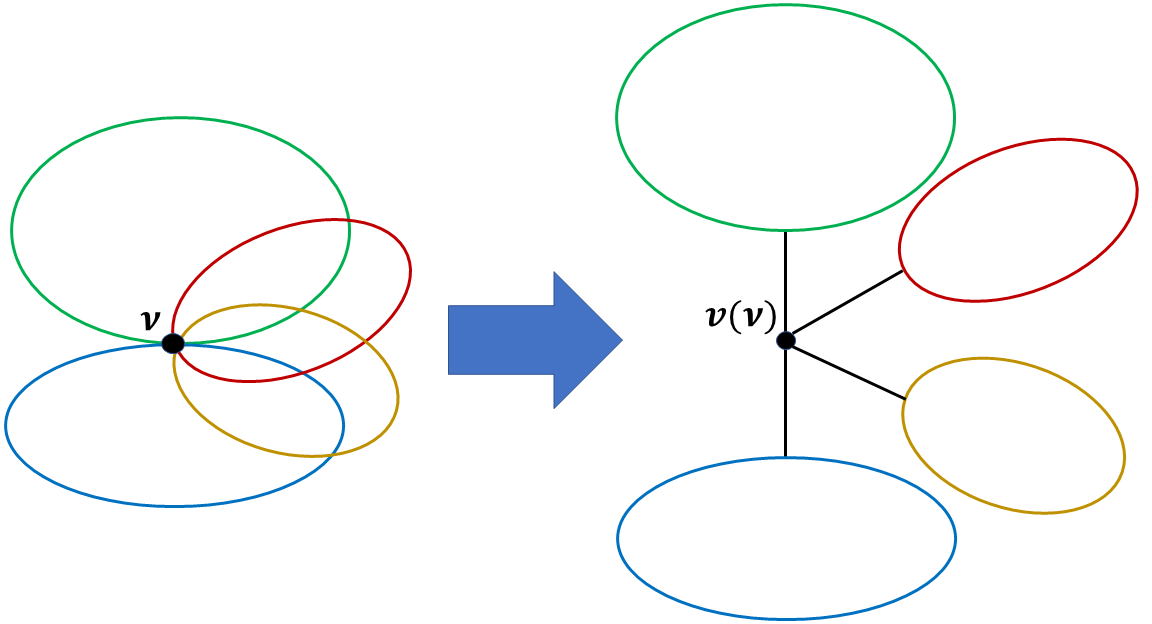
\includegraphics[width=0.6\textwidth]{src/images/Cactus-transformation.png}
    \caption{Transformation of cactus ${\cal H}_V$ to the tree $T({\cal H}_V)$.}
\label{fig:transform-cactus-to-tree}
\end{figure}

We know that if $\nu$ and $\mu$ are two nodes in the cactus, there exists a unique path of cycles and tree edges between them. It follows from the construction of $T({\cal H}_V)$ that the unique path between the vertices $v(\nu)$ and $v(\mu)$ captures the same path. Thus we state the following lemma.

\begin{lemma}
Let $\nu,\mu$ be any two arbitrary nodes in the cactus 
${\cal H}_V$. The unique path between $v(\nu)$ and $v(\mu)$ in $T({\cal H}_V)$ concisely captures all
paths between $\nu$ and $\mu$ in ${\cal H}_S$.
\label{lem:path-in-T(H_S)}
\end{lemma}

% Let $\nu$ and $\mu$ be any two nodes in skeleton ${\cal H}_S$. If they belong to the same cycle, say $c$, there are two paths between them on the cycle $c$ itself - their union forms the cycle itself. Using the fact that any two cycles in  ${\cal H}_S$ can have at most one common node, it can be seen that these are the only paths between $\nu$ and $\mu$. Using the same fact, if $\nu$ and $\mu$ belong to different cycles, there exists a unique sequence of alternating cycles and nodes $\langle \nu_1,c_1,\ldots,\nu_r,c_r,\nu_{r+1}\rangle $ satisfying the following 2 properties. \begin{itemize}
%     \item $\nu_1=\nu$, $\nu_{r+1}=\mu$, and for each $1< i\le r$, $\nu_i$ is the unique node common to $c_{i-1}$ and $c_i$.
%     \item Each path between $\nu$ and $\mu$ can be seen as a sequence $\langle p_1,\ldots p_r\rangle$ such that $p_i$ is a path between $\nu_i$ and $\nu_{i+1}$ on cycle $c_{i}$.
% \end{itemize}
% It follows from the construction of $T({\cal H}_S)$ that $\langle v(\nu_1),v(c_1),\ldots,v(\nu_r),v(c_r),v(\nu_{r+1})\rangle$ is the path between $v(\nu)$
% and $v(\mu)$. 
% Thus we can state the following lemma.
% \begin{lemma}
% Let $\nu,\mu$ be any two arbitrary nodes in the cactus 
% ${\cal H}_S$. The unique path between $v(\nu)$ and $v(\mu)$ in $T({\cal H}_S)$ concisely captures all
% paths between $\nu$ and $\mu$ in ${\cal H}_S$.
% \label{lem:path-in-T(H_S)}
% \end{lemma}

We root the tree $T({\cal H}_V)$ at any arbitrary vertex and augment it suitably so that it can answer any LCA query in $\mathcal O(1)$ time using \cite{DBLP:journals/jal/BenderFPSS05}. Henceforth, we shall use skeleton tree $T({\cal H}_S)$ to denote this data structure.

\section{Compact representation for all Steiner mincuts} \label{subsec:connectivity-carcass}

% Let $G=(V,E)$ be an undirected unweighted graph and $S\subseteq V$ be a subset (Steiner set) of its vertices. 
Dinitz and Vainshtein \cite{DBLP:conf/stoc/DinitzV94} designed a data structure $\mathfrak{C}_S = ({\cal F}_S,{\cal H}_S, \pi_S)$ that stores all the Steiner mincuts for a Steiner set $S\subseteq V$ in the graph. We present a summary of this data structure.

This data structure can be seen as a generalization of two already discussed data structures,
~(i) strip ${\cal D}_{s,t}$ storing all $(s,t)$-mincuts, and
~(ii) cactus graph ${\cal H}_V$ storing all global mincuts.

Two $S$-mincuts are said to be equivalent if they divide the Steiner set $S$ in the same way. The equivalence classes thus formed are known as the \textit{bunches}. Similarly, two vertices are said to be equivalent if they are not separated by any Steiner mincut. The equivalence classes thus formed are known as \textit{units}. A unit is called a \textit{Steiner unit} if it contains at least a Steiner vertex.

Let $(S_B,{\bar S_B})$ be the $2-$partition of Steiner set induced by a bunch $\cal B$. If we compress all vertices in $S_B$ to $s$ and all vertices in ${\bar S_B}$ to $t$, the strip ${\cal D}_{s,t}$ will store all cuts in ${\cal B}$. We shall denote this strip by ${\cal D}_{\cal B}$. Any such strip has the following property -- if two non-terminals nodes of two strips intersect at even one vertex then these nodes coincide and the inherent partitions of these nodes in both strips coincide as well.

The first component of the connectivity carcass is the \textit{flesh graph} ${\cal F}_S$ which is a generalization of the strip. This graph is a quotient graph of graph $G$. The vertices of ${\cal F}_S$ can be obtained by contracting each unit of $G$ to a single vertex. Thus, we denote the vertices of ${\cal F}_S$ simply by units. In addition to it, each unit of ${\cal F}_S$ is assigned a $2-$partition known as the \textit{inherent partition} on the set of edges incident on it. Any unit that appears as a non-terminal in the strip corresponding to some bunch is called a \textit{stretched unit}. Otherwise, it is called a \textit{terminal unit}. 
% Another distinction between these two units follows from the two observations made on strip corresponding to a bunch mentioned above. 
The inherent partition assigned to a stretched unit consists of two sets of equal cardinality. On the other hand, inherent partition assigned to a terminal unit is a trivial partition (one of the set is empty). Note that all Steiner units are terminal units but the reverse is not true.
% The concept of reachability is slightly modified in ${\cal F}_S$. Whenever we say that a unit $u$ is reachable from unit $u'$, it means that there exists a coherent path between $u$ and $u'$. A \textit{coherent path} refers to a sequence of units and edges in flesh $(u_1,e_1,u_2,e_2,\ldots,u_k)$ such that any $e_i$ is incident on $u_{i-1}$ and $u_i$ and for any $u_i$ $e_{i-1}$ and $e_i$ lie in different side of the inherent partition. The structure of the flesh graph implies that it is not possible for a coherent path to start and finish at a single unit and hence, ${\cal F}_S$ is in a sense acyclic. A \textit{transversal} refers to a $2-$partition of units such that any coherent path intersects it at most once. It can be shown that each transversal in the flesh ${\cal F}_S$ corresponds to a Steiner mincut.
The concept of reachability in ${\cal F}_S$ is similar to the strip. Whenever we say that a unit $u$ is reachable from unit $u'$, it means that there exists a coherent path between $u$ and $u'$. The structure of ${\cal F}_S$ is such that a coherent path cannot start and finish at a single unit and hence, ${\cal F}_S$ is in a sense acyclic. There is a one-to-one correspondence between transversals in ${\cal F}_S$ and Steiner mincuts in $G$.

The second component of the connectivity carcass, skeleton ${\cal H}_S$, is a cactus graph. 
To avoid confusion with the original graph, the vertices and edges of the skeleton will be referred to as nodes and structural edges respectively. 
% A structural edge in the skeleton is a tree-edge if it is not part of a cycle, otherwise, it is a cycle-edge. 
% If $c_S$ is the value of the Steiner mincut, then each tree-edge is assigned weight $c_S$ and each cycle-edge is assigned weight $\frac{c_S}{2}$. 
Each terminal unit of ${\cal F}_S$ is mapped to a node in the skeleton ${\cal H}_S$ by projection mapping ${\pi}_S$. A stretched unit on the other hand is mapped to a set of edges corresponding to a proper path in ${\cal H}_S$ by ${\pi}_S$. A \textit{proper path} in the skeleton refers to an alternating sequence of nodes and structural edges $(\nu_1,\epsilon_1,\nu_2,...,\nu_k)$ such that $\epsilon_i$ is incident on $\nu_{i-1}$ and $\nu_i$ and it intersects each cycle of the skeleton at at most one structural edge. 
% A \textit{subbunch} is a subset of a bunch that can be represented by a strip. 
All the bunches can be stored in a skeleton ${\cal H}_S$ in the form of subbunches (disjoint subsets of a bunch). Each cut in skeleton corresponds to a subbunch. The strip ${\cal D}_{\cal B}$ corresponding to this subbunch $\cal B$ can be obtained as follows. Let the cut in the skeleton separates it into two subcactuses ${\cal H}_S(\cal B)$ and ${\bar {\cal H}_S(\cal B)}$. If $P(\nu_1,\nu_2)$ be the path in the skeleton to which a unit $u$ is mapped, it will be placed in ${\cal D}_{\cal B}$ as follows.
\begin{itemize}
    \item If both $\nu_1$ and $\nu_2$ lie in ${\cal H}_S(\cal B)$ (or ${\bar {\cal H}_S(\cal B)}$) $u$ is contracted in source (or sink).
    \item Otherwise, $u$ is kept as a non-terminal unit.
\end{itemize}


Now we discuss an important property between the reachability of a stretched unit $u$ and the proper path to which it is mapped in the skeleton ${\cal H}_S$.

\begin{lemma}[\cite{DBLP:conf/soda/DinitzV95}]
Let $u$ be a stretched unit and $u'$ be any arbitrary unit in the flesh ${\cal F}_S$ and $\pi_S(u) = P(\nu_1,\nu_2)$, $\pi_S(u') = P(\nu_3,\nu_4)$. If $u'$ is reachable from $u$ in direction $\nu_2$, then both these paths are extendable to a larger proper path with $P(\nu_1,\nu_2)$ as the initial part and $P(\nu_3,\nu_4)$ as the final part.
\label{lem:path-extendable}
\end{lemma}

\begin{lemma}[\cite{DBLP:conf/stoc/DinitzV94}]
\label{lem:strip-from-carcass}
Let $s,t \in S$ such that $c_{s,t}=c_S$. Given the connectivity carcass ${\mathfrak C}_S$ storing all Steiner mincuts, the strip ${\cal D}_{s,t}$ can be constructed in time linear in the size of flesh graph.
\end{lemma}

The size of flesh ${\cal F}_S$ is ${\cal O}(\min(m,\tilde{n}c_S))$ where $\tilde{n}$ is the number of units in ${\cal F}_S$. The size taken by skeleton is linear in the number of Steiner units. Thus, overall space taken by the connectivity carcass is ${\cal O}(\min(m,\tilde{n}c_S))$.
\chapter{${\cal O}(n^2)$ space sensitivity oracle for all-pairs mincuts}


% {
% \color{blue}

% \begin{itemize}
% \item Edge-containment query for fixed s,t.
% \item Mincut containing $(x,y)$ using $(s,t)$-mincut for fixed $s,t$.
% \begin{itemize}
%     \item $O(m)$ space $O(m)$ time.
%     \item Augmented topological numbers.
%     \item $O(n)$ space $O(n)$ time.
% \end{itemize}

% \item Edge-containment query for $s,t \in S$ and $c_{s,t}=c_S$.
% \item Generalize $O(n)$ space $O(1)$ time.
% \item Mincut containing $(x,y)$ using $(s,t)$-mincut for $s,t \in S$ and $c_{s,t} = c_S$.
% \begin{itemize}
%     \item Idea of augmentation.
%     \item Given a stretched unit u and a bunch. Report the set of all stretched units that precede them in some topological ordering.
%     \item $O(n)$ space $O(n)$ time.
% \end{itemize}
% \end{itemize}
% }

% \boxed{
% $\tau$, $P$, $\pi$
% }

\section{Edge-containment query for fixed $s,t \in V$} \label{subsec:fixed-s-t}


Consider the problem of identifying if a given edge $(x,y)$ lies in a $(s,t)$-mincut for a designated pair of vertices $s,t \in V$. It is quite evident that an edge $(x,y)$ lies in a $(s,t)$-mincut if $x$ and $y$ are mapped to different nodes in the strip ${\cal D}_{s,t}$. This query can be reported in ${\cal O}(1)$ time by storing the node mapping of each vertex in ${\cal O}(n)$ space.

Reporting a $(s,t)$-mincut that contains edge $(x,y)$ requires more insights. Without loss in generality, assume that edge $(x,y)$ lies in side-$\mathbf t$ of $\mathbf x$. If $\mathbf x$ is the same as $\mathbf s$, the set of vertices mapped to node $\mathbf s$ define a $(s,t)$-mincut that contains $(x,y)$. Thus, assume that $\mathbf x$ is a non-terminal in the strip ${\cal D}_{s,t}$. It is important to observe that set of vertices mapped to nodes in the reachability cone of $\mathbf x$ towards $\mathbf s$, ${\cal R}_s({\mathbf x})$, defines a $(s,t)$-mincut that contains edge $(x,y)$. However, reporting this mincut requires ${\cal O}(m)$ time and ${\cal O}(m)$ space. 
% Assuming Conjecture \ref{conj:directed-reachability-hypothesis} holds, any improvement in query time would require ${\Omega}(n^2)$ space.

To achieve better space and query time, we report another $(s,t)$-mincut that contains $(x,y)$ and has a simpler structure. Suppose $\tau$ is a topological ordering on the node set of strip ${\cal D}_{s,t}$ with $\tau(\mathbf s) = 0$. We show that storing the node mapping of each vertex and topological number of each node $\tau$ of the strip ${\cal D}_{s,t}$ can be used to report a $(s,t)$-mincut efficiently. 
% Consider the set of nodes, $X = \{u \;|\; \tau(u) \leq \tau(\mathbf x)\}$, with topological numbers less than or equal to that of $\mathbf x$. The set of vertices mapped to nodes in $X$ defines one such $(s,t)$-mincut. 
This data structure takes only ${\cal O}(n)$ space and can report a $(s,t)$-mincut containing edge $(x,y)$ in ${\cal O}(n)$ time. We state the following lemma.

\begin{lemma}
\label{lem:s-t-mincut-containing-x-y-topological-fixed}
Consider the strip ${\cal D}_{s,t}$ with ${\mathbf x}$ as a non-terminal, and edge $(x,y)$ lies on side-${\mathbf t}$ of ${\mathbf x}$. Suppose $\tau$ is a topological order on the nodes in the strip. The set of vertices mapped to nodes in set $X = \{u \;|\; \tau(u) \leq \tau(\mathbf x)\}$ defines a $(s,t)$-mincut that contains edge $(x,y)$.
\end{lemma}

\section{Edge-containment query for Steiner set $S$} \label{subsec:edge-containment-ds-steiner}

Suppose $S$ is a designated Steiner set and $s,t\in S$ are Steiner vertices separated by some Steiner mincut. We can determine if an edge $(x,y)\in E$ belongs to some $(s,t)$-mincut using the strip ${\cal D}_{s,t}$ that can be built from the connectivity carcass. However, the construction of strip requires ${\cal O}(\min(m,nc_S))$ time. Interestingly, we show that only the skeleton and the projection mapping of the connectivity carcass are sufficient for answering this query in constant time. Moreover, the skeleton and the projection mapping occupy only ${\cal O}(n)$ space compared to the ${\cal O}(\min(m,nc_S))$ space occupied by the entire connectivity carcass.

Similar to the projection mapping of the stretched units, Dinitz and Vainshtein \cite{DBLP:journals/siamcomp/DinitzV00} introduced the notion of projection mapping for edges as follows. Suppose $(x,y)\in E$. If $x$ and $y$ belong to the same unit, then $P(x,y) = \varnothing$. If $x$ and $y$ belong to distinct terminal units mapped to nodes, say $\nu_1$ and $\nu_2$, in the skeleton ${\cal H}_S$, then $P(x,y) = P(\nu_1,\nu_2)$. If at least one of them belongs to a stretched unit, $P(x,y)$ is the extended path defined in Lemma \ref{lem:path-extendable}. This allows us to state the following lemma which follows from the construction of a strip corresponding to a subbunch given in Section \ref{subsec:connectivity-carcass}.

\begin{lemma}[\cite{DBLP:conf/stoc/DinitzV94}]
Edge $(x,y)\in E$ appears in the strip corresponding to a subbunch if and only if one of the structural edge in the cut of ${\cal H}_S$ corresponding to this subbunch lies in $P(x,y)$.
\label{lem:edge-path-intersect-subbunch}
\end{lemma}

We state the necessary and sufficient condition for an edge $(x,y)$ to lie in an $(s,t)$-mincut. Note that two paths are said to intersect in the skeleton if the unique path of cycle and tree edges in both the paths intersect at some cycle or tree edge.
% The skeleton ${\cal H}_{S(\nu)}$ and the corresponding projection mapping $\pi_{S(\nu)}$ have the sufficient information to infer whether any edge $(x,y)\in E$ belongs to some $(s,t)$-mincut as stated by the following lemma. We say that two paths intersect if the unique path of cycle and tree edges in both the paths intersect at some cycle or tree edge.

\begin{lemma} \label{lem:path-intersects-tree}
 Edge $(x,y)\in E$ belongs to a $(s,t)$-mincut if and only if the proper path $P(x,y)$ intersects a path between the nodes containing $s$ and $t$ in in $\mathcal H_{S}$.
\end{lemma}
\begin{proof}

% {\color{blue} make it short.}

% Observe that an edge $(x,y)$ lies in a $(s,t)$-mincut if and only if it appears in the strip ${\cal D}_{s,t}$ (follows from Lemma \ref{lem:E_y-edges-same-side}). Infact, we can extend this notion for subbunch as well. The edge $(x,y)$ lies in some $(s,t)$-mincut if and only if it appears in the strip corresponding to some subbunch that separates $s$ from $t$.

% Consider each subbunch that separates $s$ from $t$.

Let $\nu_1$ and $\nu_2$ be the nodes in ${\cal H}_S$ containing $s$ and $t$ respectively. A cut in ${\cal H}_S$ corresponding to any tree-edge (or pair of cycle edges in same cycle) in the path from $\nu_1$ to $\nu_2$ defines a subbunch separating $s$ from $t$. Moreover, it follows from the structure of the skeleton that no other cut in the skeleton corresponds to a subbunch separating $s$ from $t$. Suppose $(x,y)$ lies in some $(s,t)$-mincut. Thus, it must be in some subbunch separating $s$ from $t$. From the above discussion, we know that this subbunch must correspond to a cut in the path from $\nu_1$ to $\nu_2$ in skeleton ${\cal H}_S$. Moreover, it follows from Lemma \ref{lem:edge-path-intersect-subbunch} that $P(x,y)$ contains one of the structural edge in this cut. This implies that $P(x,y)$ intersects the path from $\nu_1$ to $\nu_2$ in skeleton ${\cal H}_S$.

Now, consider the other direction of this proof. Suppose $P(x,y)$ and the path from $\nu_1$ to $\nu_2$ intersect at some cycle (or tree edge) $c$. Let $e_1$ and $e_2$ be structural edges belonging to the cycle $c$ that are part of $P(x,y)$ and path from $\nu_1$ to $\nu_2$ respectively (in the case of tree edge $e_1=e_2=c$). Consider the cut in the skeleton corresponding to structural edges $e_1$ and $e_2$. It follows from Lemma \ref{lem:edge-path-intersect-subbunch} that $(x,y)$ lies in the strip corresponding to this subbunch. Since this cut separates $\nu_1$ from $\nu_2$ in ${\cal H}_S$, therefore the subbunch separates $s$ from $t$.
\end{proof}

We can check if paths $P(\nu_1,\nu_2)$ and $P(s,t)$ in the skeleton ${\cal H}_S$ intersect with ${\cal O}(1)$ LCA queries on skeleton tree ${\cal T}({\cal H}_S)$ (using Lemma \ref{lem:xyz}). Thus, we can store the skeleton tree ${\cal T}({\cal H}_S)$ and projection mapping in ${\cal O}(n)$ space and determine if an edge $(x,y)$ lies in an $(s,t)$-mincut for $c_{s,t}=c_S$ and $s,t \in S$ in ${\cal O}(1)$ time.


Reporting a $(s,t)$-mincut that contains edge $(x,y)$ again requires more insights. Assume that $P(s,t)$ and $P(\nu_1,\nu_2)$ intersect at some tree edge or cycle. Let $e$ be a tree or cycle-edge in proper path $P(\nu_1,\nu_2)$ that lies in intersection of these two paths. Suppose ${\cal B}$ is a subbunch corresponding to a cut in the skeleton ${\cal H}_S$ that contains $e$ and separates $s$ from $t$ and ${\cal D}_{\cal B}$ be the strip corresponding to this subbunch. Without loss in generality, assume that $\nu_1$ lies in the side of source $s$ in this strip (denoted by ${\mathbf s}$). Using Lemma \ref{lem:edge-path-intersect-subbunch}, it is evident that edge $(x,y)$ lies in strip ${\cal D}_{\cal B}$. Assume $\mathbf x$ is a stretched unit in this strip, otherwise the source $\mathbf s$ is the required $(s,t)$-mincut. Suppose $(x,y)$ lies in side-$\mathbf t$ of $\mathbf x$. The set of vertices mapped to ${\cal R}_s(\mathbf{x})$, i.e. reachability cone of $\mathbf x$ towards $\mathbf s$ in this strip, defines a $(s,t)$-mincut that contains edge $(x,y)$. However, reporting this mincut is a tedious task. We must have the flesh ${\cal F}_S$ to construct the strip ${\cal D}_{\cal B}$ and then report the set ${\cal R}_s(\mathbf{x})$. This would require ${\cal O}(m)$ space and ${\cal O}(m)$ time.

It is important to observe that the difficulty we face here is similar to the one highlighted in Section \ref{subsec:fixed-s-t}. To achieve better space and query time, we use similar ideas as used in Section \ref{subsec:fixed-s-t}. We aim to report another $(s,t)$-mincut that contains $(x,y)$ and has a simpler structure. In particular, we aim to report a set of units $X = \{ u \;|\; \tau_{\cal B}(u)\leq \tau_{\cal B}(\mathbf{x})\}$ for some topological ordering $\tau_{\cal B}$ of nodes in strip ${\cal D}_{\cal B}$. Using Lemma \ref{lem:s-t-mincut-containing-x-y-topological-fixed}, we know that set of vertices mapped to nodes in set $X$ defines a $(s,t)$-mincut that contains edge $(x,y)$. Clearly, storing topological order for each stretched unit for each possible bunch in which it appear as a non-terminal is not an option. This is because doing so will require a lot of space. Thus, we try to devise an algorithm to efficiently identify set $X$ on without compromising ${\cal O}(n)$ size of the data structure.

Consider the data structure formed by the following components -- ~(i) the skeleton tree ${\cal T}({\cal H}_S)$, ~(ii) the projection mapping $\pi_S$ of all units and ~(iii) a mapping $\tau$ from each stretched unit to a number. For all stretched units mapped to path $P(\nu_1,\nu_2)$, $\tau$ assigns a topological order on these stretched units as they appear in the $(\nu_1,\nu_2)$-strip. We now show how this additional augmentation will help us report a $(s,t)$-mincut containing edge $(x,y)$ efficiently.


In order to make the ideas more simple, we describe a transitive relation between proper paths on skeleton called \textit{extendable in a direction}.


% {\color{red} extendable in direction $\nu_2$ looks a bit. Try to redefine only in terms of projection mapping paths.}
% \subsubsection{Extendable in a direction}
\begin{definition}[Extendable in a direction]
% Suppose $u$ and $v$ are two stretched units projected to proper paths $P(\nu_1,\nu_2)$ and $P(\nu_3,\nu_4)$ respectively. $v$ is said to be extendable in direction $\nu_2$ of $u$ if proper paths $P(\nu_1,\nu_2)$ and $P(\nu_3,\nu_4)$ are extendable to a proper path $P(\nu,\nu')$ with $P(\nu_1,\nu_2)$ as the initial part and $P(\nu_3,\nu_4)$ as the final part.
Consider two proper paths $P_1 = P(\nu_1,\nu_2)$ and $P_2 = P(\nu_3,\nu_4)$. $P_2$ is said to be extendable from $P_1$ in direction $\nu_2$ if proper paths $P_1$ and $P_2$ are extendable to a proper path $P(\nu,\nu')$ with $P_1$ as the initial part and $P_2$ as the final part.
\label{def:extendable}
\end{definition}

% It follows from Theorem \ref{lem:path-extendable} that if the stretched unit $v$ is reachable from $u$ in the direction $\nu_2$ through a coherent path, then $v$ is extendable in direction $\nu_2$ from $u$.
Moreover, verifying if $P(\nu_3,\nu_4)$ is extendable from $P(\nu_1,\nu_2)$ in direction $\nu_2$ can be done in ${\cal O}(1)$ LCA queries on the skeleton tree.


Suppose stretched unit $\mathbf x$ is mapped to path $P(\nu,\nu')$. Consider the set $X$ formed by stretched units appearing as non-terminals in strip ${\cal D}_{\cal B}$ for which one of the following holds true -- (i) the stretched unit (say $v$) is mapped to $P(\nu,\nu')$ and $\tau(v) \leq \tau(\mathbf x)$, and (ii) the stretched unit is not mapped to $P(\nu,\nu')$ but $\pi_S(v)$ is extendable from $P(\nu,\nu')$ in direction $\nu$. We state the following lemma.

\begin{lemma}
The vertices mapped to units in ${\mathbf s}\cup X$ define a $(s,t)$-mincut and contains all the edges in side-$\mathbf t$ of the inherent partition of $\mathbf x$.
\end{lemma}
\begin{proof}
Consider $u \in X$ to be a non-terminal unit in ${\cal D}_{\cal B}$. We shall show that ${\cal R}_{\mathbf s}(u)\setminus \mathbf{s} \subseteq X$, i.e. reachability cone of $u$ towards source $\mathbf{s}$ in the strip ${\cal D}_{\cal B}$ avoiding $\mathbf s$ is a subset of $X$. It follows from the construction that $u$ is either projected to $P(\nu,\nu')$ or $\pi_S(u)$ is extendable in direction $\nu$ from $P(\nu,\nu')$. Consider any unit $v$ in ${\cal R}_{\mathbf s}(u)\setminus \mathbf{s}$. Suppose $u$ and $v$ are both projected to $P(\nu,\nu')$. Since, $v$ is reachable from $u$ in direction $\nu$, it follows that $\tau(v) < \tau(u) < \tau(\mathbf{x})$. Thus, $v \in X$. Now, suppose $v$ is not projected to $P(\nu,\nu')$. In this case, $\pi_S(v)$ is extendable from $P(\nu,\nu')$ in direction $\nu$ (from Theorem \ref{lem:path-extendable}). It follows from the transitivity of Definition \ref{def:extendable} that $\pi_S(v)$ is extendable from $\pi_S(u)$ in direction $\nu$. Thus, $v \in X$. Therefore, ${\mathbf s}\cup X$ defines a $(s,t)$-mincut (from Lemma \ref{lem:mincut-transversal}).

Now, we prove the second part of the lemma. Consider any edge $(x,z)$ in the side-$\mathbf{t}$. If $z$ is in $\mathbf t$ then $z \not \in X$ from the construction. Assume that $z$ is a non-terminal unit in ${\cal D}_{\cal B}$. If $z$ is projected to path $P(\nu,\nu')$ then $\tau(z) > \tau(u)$. Thus, $z \not \in X$. Otherwise $\pi_S(z)$ is extendable from $P(\nu,\nu')$ in direction $\nu'$. It follows from Definition \ref{def:extendable} that $z \not \in X$. Thus, the cut defined by ${\mathbf s} \cup X$ contains all edges in side-$\mathbf{t}$ of the inherent partition of $\mathbf x$.

\end{proof}

This data structure occupies ${\cal O}(n)$ space and can report a $(s,t)$-mincut containing edge $(x,y)$ in ${\cal O}(n)$ time. We shall use this data structure to build a sensitivity oracle for all-pairs mincuts.


\section{Edge-containment query for all-pairs Mincuts}

The hierarchical tree structure of Katz, Katz, Korman and Peleg \cite{DBLP:journals/siamcomp/KatzKKP04} can be suitably augmented to design a sensitivity oracle for all-pairs mincuts. We augment each internal node $\nu$ of the hierarchy tree ${\cal T}_G$ by the data structure discussed in Section \ref{subsec:edge-containment-ds-steiner} for the Steiner set $S(\nu)$. Determining if given edge $(x,y)$ lies in some $(s,t)$-mincut for given pair of vertices $s,t\in V$ can be done using Algorithm \ref{algo:quadratic-space-query} in constant time. 

\begin{algorithm}%[H]
    \caption{Single edge-containment queries in ${\cal O}(n^2)$ data structure}
    \label{algo:quadratic-space-query}
    \begin{algorithmic}[1] % The number tells where the line numbering should start
        \Procedure{edge-cotained}{$s,t,x,y$}
            \State{${\mu}\gets$ LCA($\mathcal T_G,s,t$)}
            \State $\mathcal P_1 \gets P(\pi_{S(\mu)}(s),\pi_{S(\mu)}(t))$
            \State $\mathcal P_2 \gets P(x,y)$
            \If{$\mathcal P_1 \cap \mathcal P_2 = \varnothing$} \Comment{Check if paths intersect} 
            \State \textbf{return} False
            \Else 
            \State \textbf{ return} True
            \EndIf
        \EndProcedure
    \end{algorithmic}
\end{algorithm}


% We state the following theorem.

% We build our data structure using the findings of Lemma \ref{lem:path-intersects-tree}. We augment each internal node $\mu$ of the hierarchy tree ${\cal T}_G$ with the skeleton tree $T({\cal H}_{S(\mu)})$ and the projection mapping ${\pi}_{S(\mu)}$ corresponding to Steiner set $S(\mu)$. In addition to it, for each stretched unit $u$ mapped to path $P(\nu_1,\nu_2)$ in skeleton ${\cal H}_{S(\mu)}$ we also store a number ${\tau(u)}$ that denotes the topological order of $u$ as it appears in the $(\nu_1,\nu_2)$-strip.  This additional information will help us efficiently report the mincut upon failure of an edge. Since augmentation at each internal node takes ${\cal O}(n)$ space, therefore the total space occupied by the data structure is only ${\cal O}(n^2)$.


% Consider any node $\nu$ in ${\cal T}_G$.
% Let $s,t$ be any two vertices such that
% $\nu$ is their LCA in ${\cal T}_G$. $s$ and $t$ must belong to different nodes in the the skeleton ${\cal H}_{S(\nu)}$ stored at $\nu$. 
% It follows from Lemma \ref{lem:path-intersects-tree} that for a single-edge-containment query, we just have to keep the skeleton tree and the projection mapping at each internal node in ${\cal T}_G$. It is important to note that both these data structures collectively only take up ${\cal O}(n)$ space, contrary to the ${\cal O}(\min(m,nc_S)$ size taken up by the entire connectivity carcass. Thus, the size taken up by complete data structure is only ${\cal O}(n^2)$. 

% \section{Edge-containment Query on Data Structure}
% Determining whether a given edge belongs to a $(s,t)$-mincut can be done as follows. Let $\mu$ be the LCA of $s$ and $t$ in ${\cal T}_G$. It follows from Observation \ref{obs:(s,t)-mincut-lca} that $c_{s,t}=c_{S(\mu)}$. Thus, $s$ and $t$ must be separated by some Steiner mincut for set $S(\mu)$. We check if paths $P(x,y)$ and $P(\pi_{S(\mu)}(s),\pi_{S(\mu)}(t))$ intersect in the skeleton ${\cal H}_{S(\mu)}$ (using Lemma \ref{lem:path-intersects-tree}). This can be done using ${\cal O}(1)$ LCA queries on the skeleton tree $T({\cal H}_{S(\mu)})$. Since it takes ${\cal O}(1)$ time for answering one LCA query \cite{DBLP:journals/jal/BenderFPSS05}, so the query time will be only ${\cal O}(1)$. Algorithm \ref{algo:quadratic-space-query} presents a concise pseudocode of the query answering algorithm.




% Now, we show how to report an $(s,t)$-mincut which contains the edge $(x,y)$ in ${\cal O}(n)$ time. 

% In order to make the ideas more simple, we describe a transitive relation between stretched units called \textit{extendable in a direction}.

% \begin{definition}[Extendable in a direction]
% Suppose $u$ and $v$ are two stretched units projected to proper paths $P(\nu_1,\nu_2)$ and $P(\nu_3,\nu_4)$ respectively. $v$ is said to be extendable in direction $\nu_2$ of $u$ if proper paths $P(\nu_1,\nu_2)$ and $P(\nu_3,\nu_4)$ are extendable to a proper path $P(\nu,\nu')$ with $P(\nu_1,\nu_2)$ as the initial part and $P(\nu_3,\nu_4)$ as the final part.
% % \label{def:extendable}
% \end{definition}

% It follows from Theorem \ref{lem:path-extendable} that if the stretched unit $v$ is reachable from $u$ in the direction $\nu_2$ through a coherent path, then $v$ is extendable in direction $\nu_2$ from $u$. Moreover, verifying if $v$ is extendable from $u$ in direction $\nu_2$ can be done in ${\cal O}(1)$ LCA queries on the skeleton tree.

% Suppose $s,t \in S$ are steiner vertices such that $c_{s,t}=c_S$ and $u$ is a stretched unit mapped to path $P(\nu_1,\nu_2)$. Moreover, it is known that $P(s,t)$ and $P(\nu_1,\nu_2)$ intersect at some tree edge or cycle. Let $e$ be a tree or cycle-edge in proper path $P(\nu_1,\nu_2)$ that. Our task is to report a $(s,t)$-mincut that contains all the edges in one side of the inherent partition of $u$ (say side-$\nu_2$). Suppose ${\cal B}$ is a subbunch corresponding to a cut in the skeleton ${\cal H}_S$ that contains $e$ and separates $s$ from $t$. Without loss in generality, assume that $\nu_1$ lies in the side of $s$ in this cut (denoted by ${\mathbf s}$). It follows from the construction that $u$ is a non-terminal unit in the strip ${\cal D}_{\cal B}$. Assume that side of $s$ is the source in this strip. 

% % To report a $(s,t)$-mincut containing all edges in side-$\nu_2$ of $u$, it suffices to report all non-terminal units in strip ${\cal D}_{\cal B}$ that precede $u$ in the topological ordering. It is important to note that multiple topological ordering may exist for this strip, but any one of them shall work in this case.

% Consider the set $U$ formed by stretched units appearing as non-terminals in strip ${\cal D}_{\cal B}$ for which at one of the following holds true -- (i) the stretched unit (say $v$) is mapped to $P(\nu_1,\nu_2)$ and $\tau(v) \leq \tau(u)$, and (ii) the stretched unit is not mapped to $P(\nu_1,\nu_2)$ but is extendable from $u$ in direction $\nu_1$. We state the following lemma.

% \begin{lemma}
% The vertices mapped to units in ${\mathbf s}\cup U$ define a $(s,t)$-mincut that contains all the edges in side-${\nu}_2$ of the inherent partition of $u$.
% \end{lemma}
% \begin{proof}
% Consider $x \in U$ to be a unit. We shall show that ${\cal R}_{\mathbf s}(x)\setminus \mathbf{s} \subseteq U$. It follows from the construction that $x$ is either projected to $P(\nu_1,\nu_2)$ or is extendable in direction $\nu_1$ from $x$. Consider any unit $y$ in ${\cal R}_{\mathbf s}(x)\setminus \mathbf{s}$. Suppose $x$ and $y$ are both projected to $P(\nu_1,\nu_2)$. Since, $y$ is reachable from $x$ in direction $\nu_1$, it follows that $\tau(y) < \tau(x) < \tau(u)$. Thus, $y \in U$. Now, suppose $y$ is not projected to $P(\nu_1,\nu_2)$. In this case, $y$ is extendable from $x$ in direction $\nu_1$ (from Theorem \ref{lem:path-extendable}). It follows from the transitivity of Definition \ref{def:extendable} that $y$ is extendable from $u$ in direction $\nu_1$. Thus, $y \in U$.

% Now, we prove the second part of the lemma. Consider any edge $(u,w)$ in the side-$\nu_2$. If $w$ is in $\mathbf t$ then $w \not \in U$ from the construction. Assume that $w$ is a non-terminal unit in ${\cal D}_{\cal B}$. If $w$ is projected to path $P(\nu_1,\nu_2)$ then $\tau(w) > \tau(u)$. Thus, $w \not \in U$. Otherwise $w$ is extendable from $u$ in direction $\nu_2$. It follows from Definition \ref{def:extendable} that $w \not \in U$. Thus, the cut defined by ${\mathbf s} \cup U$ contains all edges in side-$\nu_2$ of the inherent partition of $u$.

% \end{proof}

% Now, consider the case when at least one of $x$ and $y$ belongs to a stretched unit. In this case, we can use the above ideas to report the $(s,t)$-mincut containing this edge. If both $x$ and $y$ belong to different terminal units, then simply reporting the terminal unit $\mathbf{s}$ of ${\cal D}_{\cal B}$ will suffice.


\section{Edge-insertion query on Data Structure}

Determining whether insertion of an edge $(x,y)$ increases the $(s,t)$-mincut is comparatively simpler. Again, let $\mu$ be the LCA of $s$ and $t$ in ${\cal T}_G$. For sake of simplicity, assume that $x,y,s$ and $t$  be units in flesh graphs corresponding to vertices $x,y,s$ and $t$ respectively. Using Lemma \ref{lem:edge-insertion-increases-mincut}, we only need to determine if $x \in s_t^N$ and $y \in t_s^N$ or vice-versa. Using Lemma \ref{lem:u-nearest-s-t-mincut}, we can perform this operation in ${\cal O}(1)$ time. Reporting $(s,t)$-mincut after insertion of an edge can be done in ${\cal O}(n)$ time (using Lemma \ref{lem:u-nearest-s-t-mincut}) as $s_t^N$ is one such mincut. Thus, we can summarize the results of previous two sections in the following theorem.

\begin{theorem}
Given an undirected unweighted multigraph $G=(V,E)$ on $n=|V|$ vertices, there exists an
${\cal O}(n^2)$ size sensitivity oracle that can report the value of $(s,t)$-mincut for any $s,t \in V$ upon insertion/deletion of an edge. A $(s,t)$-mincut incorporating the insertion/deletion can be reported in ${\cal O}(n)$ time.
\label{thm:O(n^2)-size-data-structure}
\end{theorem}
\chapter{Compact Graph for Query Transformation}
\label{sec:compact-graph-section}
Let $S\subseteq V$ be the Steiner set of vertices. Suppose $S'\subset S$ be any maximal subset of vertices with connectivity greater than that of $S$.  Observe that the entire set $S'$ will be mapped to a single node, say $\nu$, in the skeleton ${\cal H}_S$. In this section, we present the construction of a compact graph $G_{S'}$ such that any query \textsc{edge-contained}$(s,r,E_y)$ in graph $G$ can be efficiently transformed to a query \textsc{edge-contained}$(s,r,E_{y'})$ in graph $G_{S'}$ for any $s,r\in S'$.
% on which can answer \textsc{edge-contained}$(s,r,E_y)$ efficiently for any $s,r\in S'$ and any subset $E_y$ of edges emanating from $y\in V$.
\vspace{-2mm}
\section{Construction of Compact Graph \texorpdfstring{$G_{S'}$}{}}\label{sec:compact-graph}


The construction of $G_{S'}$ from the graph $G$, flesh ${\cal F}_S$ and skeleton ${\cal H}_S$ is a $2-$step process. In the 1st step, we contract the subcactuses neighbouring to node $\nu$ using the following procedure.
%We start with the original graph and then contract the subcactuses using the following procedure,

{\textsc{Contract-Subcactuses}}: For each tree-edge incident on $\nu$ (or cycle $c$ passing through $\nu$) in skeleton ${\cal H}_S$, remove the tree-edge (or the pair of edges from $c$ incident on $\nu$) to get 2 subcactuses. Compress all the terminal units of ${\cal F}_S$ that belong to the subcactus not containing $\nu$ into a single vertex. Moreover, compress all the stretched units with both endpoints within this subcactus into the same vertex.

In the quotient graph obtained after 1st step, each contracted subcactus defines a Steiner mincut. 
However, this graph may not necessarily be compact since there may be many stretched units that are not yet compressed. 
%Consider one such stretched unit $u$ and suppose
Let $u$ be any such unit and suppose
the path to which it is mapped in the skeleton is $P(\nu_1,\nu_2)$. If one of $\nu_1$ or $\nu_2$ is $\nu$, we can compress the stretched unit to the contracted vertex corresponding to the other endpoint. To handle the case when the subcactuses containing $\nu_1$ and $\nu_2$ are compressed to different vertices,
%The challenge is to tackle the case when subcactuses containing $\nu_1$ and $\nu_2$ are compressed to different vertices. 
% At first sight, it may seem appropriate to arbitrarily compress such stretched unit to one of these vertices. However, this approach won't guarantee that the contracted subcactus corresponds to a Steiner mincut. It can be explained as follows. Suppose $u_1,u_2$ and $u_3$ are three stretched units and there is a coherent path in ${\cal F}_S$ that passes through them in the order $\langle u_1,u_2,u_3 \rangle$. If we compress $u_2$ to one vertex and $u_1,u_3$ to another, the cut defined by either of these vertices will intersect the coherent path twice, and hence it will not be a Steiner mincut.
%To tackle this problem,
we define a total ordering on the set containing all tree-edges and cycles in the skeleton. The 2nd step uses this ordering to compress the stretched units as follows.
%Thenceforth, we contract each of the remaining stretched units to one of the contracted subcactus using the following procedure to get $G_{S'}$,


{\textsc{Contract-Stretched-Units}}: A stretched unit mapped to path $P(\nu_1,\nu_2)$, where $\nu_1\neq \nu \neq \nu_2$, is compressed to the contracted subcactus corresponding to lesser ordered cycle/tree-edge in which endpoints lie. If one of $\nu_1$ or $\nu_2$ is $\nu$, we compress it to the contracted subcactus corresponding to the cycle/tree-edge where other endpoint lies.

Figure \ref{fig:image-contraction} gives a nice illustration of the contraction procedure.

\begin{figure}
    \centering
    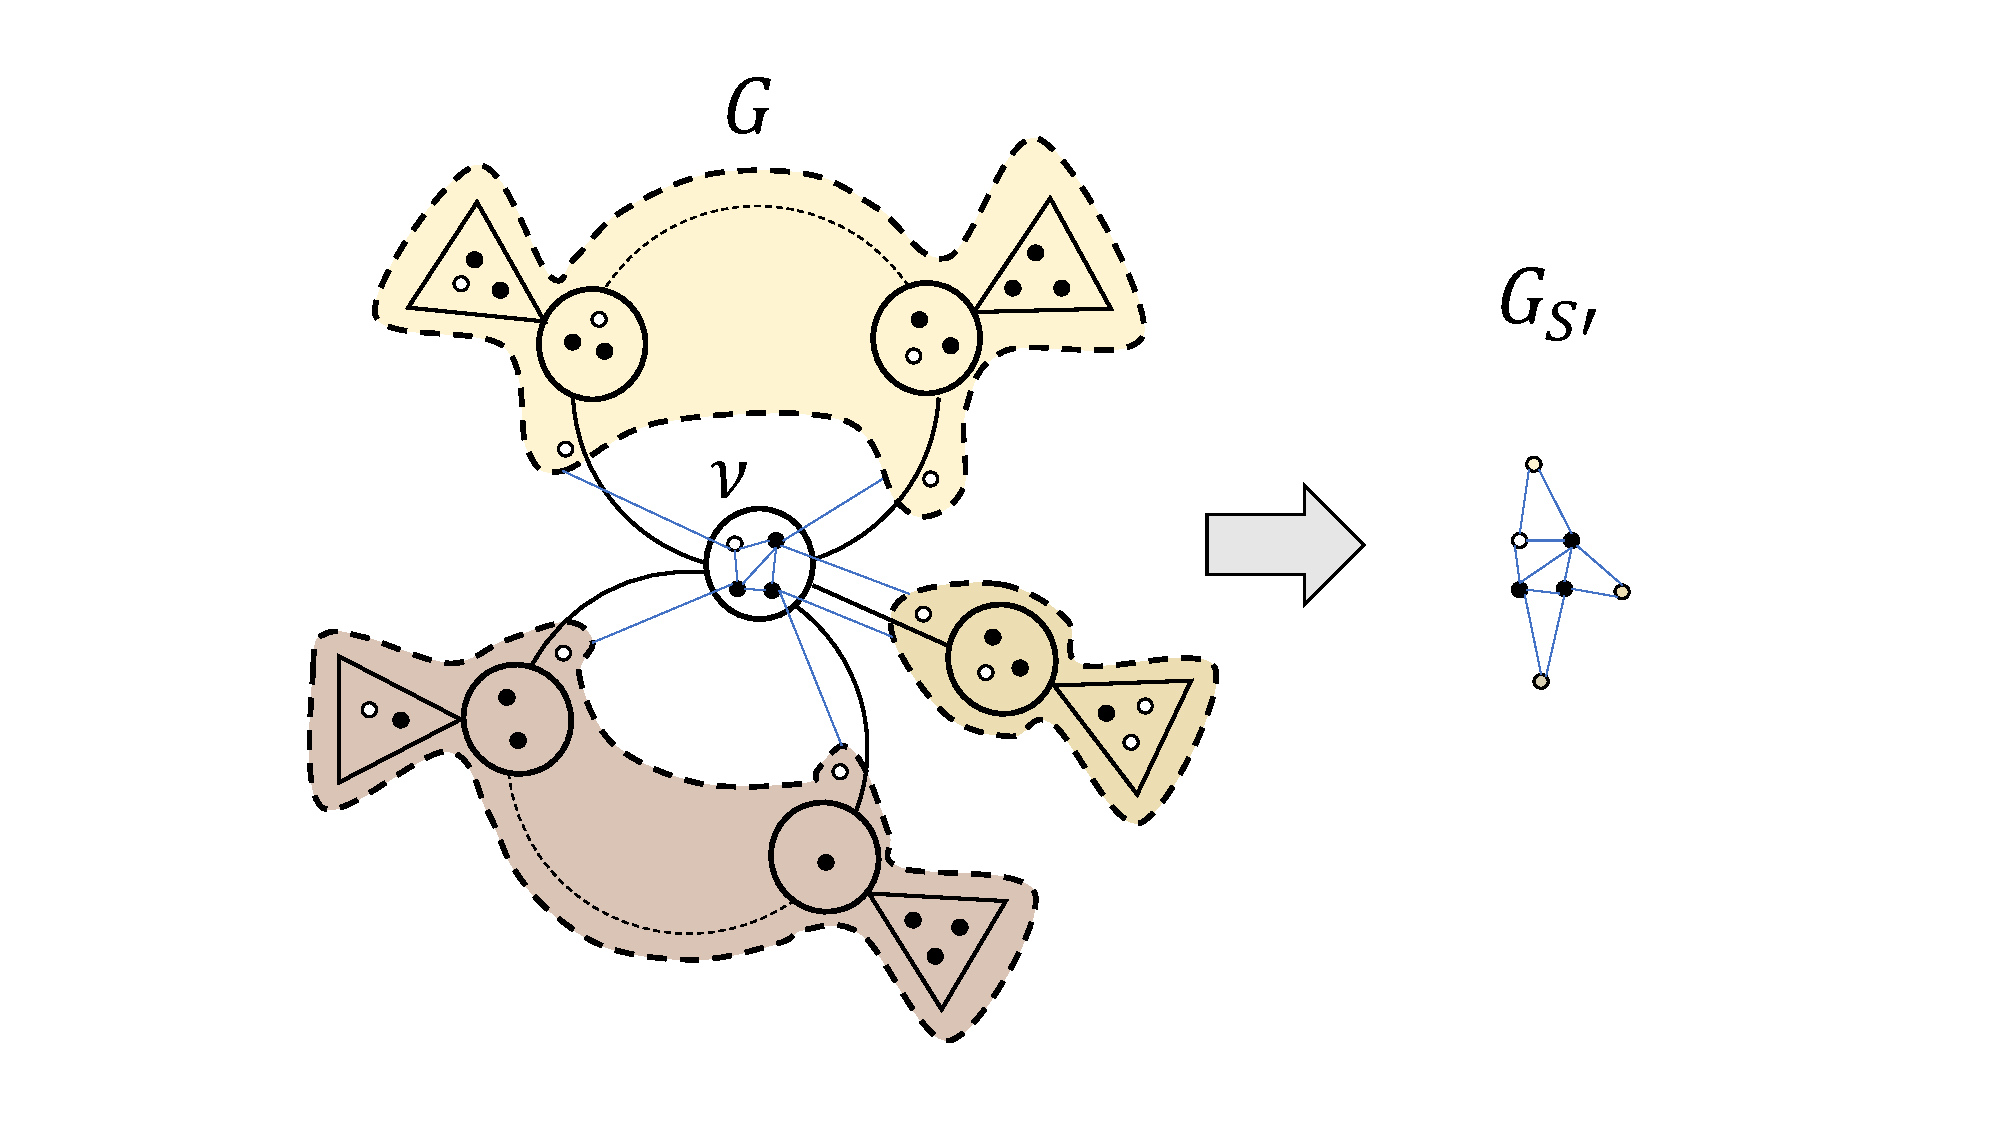
\includegraphics[width=\textwidth]{src/images/image_contraction.pdf}{}
    \caption{$2$-step contraction procedure to construct $G_{S'}$. We only show the vertices and relevant edges of graph along with the skeleton ${\cal H}_S$. Solid vertices belong to Steiner set $S$ and hollow vertices are non-Steiner vertices. All Steiner vertices inside node $\nu$ form the set $S'$.}
    \label{fig:image-contraction}
\end{figure}


Let $c$ be any cycle (or tree edge) passing through (incident on) $\nu$ in the skeleton
${\cal H}_S$. Let ${\cal D}_{s,t}$ be the strip corresponding to the sub-bunch defined by the structural edge(s) incident on $\nu$ by $c$.
Let $\nu$ be on the side of the source $\mathbf{s}$ in this strip.
Let ${\cal H}_S(c)$ be the subcactus formed by removing the structural edge(s) from $c$ incident on $\nu$ and not containing $\nu$. 
Recall that the subcactus ${\cal H}_S(c)$ was contracted into a vertex, say $v_c$, in the graph 
$G_{S'}$.
%Moreover, suppose $v_c$ is the contracted vertex corresponding to contracted subcactus ${\cal H}_S(c)$.
%Also, assume that $\nu$ is on the side of the source $\mathbf{s}$ in this sub-bunch.

\begin{lemma}
Let $u$ and $u'$ be any two non-terminal units in ${\cal D}_{s,t}$ such that none of them is compressed to $v_c$ in $G_{S'}$. If one of them is reachable from the other in the direction of ${\mathbf{s}}$, then both of them will be compressed to the same contracted vertex in $G_{S'}$.
%
%Let $u$ and $u'$ be any two non-terminal units in ${\cal D}_{s,t}$ such that $u'$ is reachable from $u$ in the direction of ${\mathbf{s}}$ and $u$ is not contracted to vertex $v_c$. $u'$ and $u$ will be compressed to the same contracted node in $G_{S'}$.
\label{lem:u-u'-in-G-nu}
\end{lemma}
\begin{proof}
Assume without loss of generality that $u'$ is reachable from $u$ in the direction of ${\mathbf{s}}$.
Let the proper paths associated with each of $u$ and $u'$ in ${\cal H}_S$ be $P(\nu_1,\nu_2)$ and $P(\nu_1',\nu_2')$ respectively. 
It follows from the construction of ${\cal D}_{s,t}$ that
$P(\nu_1,\nu_2)$ as well as $P(\nu_1',\nu_2')$ will pass through one of the structural edge(s) from $c$ on $\nu$. Without loss of generality,  assume that $P(\nu_1,\nu_2)$ passes through $e$. Since $P(\nu_1,\nu_2)$ is a proper path, this implies that this is the only structural edge in this cut (of skeleton) through which this path passes.
Since $u'$ is reachable from $u$ in flesh ${\cal F}_S$, so $P(\nu_1',\nu_2')$ will also have to pass through $e$ (from Lemma \ref{lem:path-extendable}).
It again follows from Lemma \ref{lem:path-extendable}, that $P(\nu_1,\nu_2)$ as well as $P(\nu_1',\nu_2')$ are subpaths of a path, say $P(\nu',\nu'')$, in skeleton
${\cal H}_S$. This combined with the above discussion establishes that $P(\nu',\nu'')$ has the structure shown in Figure \ref{fig:structure-of-p(nu',nu'')}.

Observe that any path in skeleton that passes through a node $\nu$ can intersect at most 2 cycles or tree-edges that are passing though $\nu$. We know that suffix of $P(\nu',\nu'')$ after $e$ lies in ${\cal H}_S(c)$, so the prefix upto $e$ must have endpoint in subcactus ${\cal H}_S(c')$ where $c'\neq c$. This implies that $u$ must be compressed to $v_{c'}$ because it is not compressed to $v_c$. Thus, $c'$ precedes $c$ in total order. It follows from the structure of path $P(\nu_1',\nu_2')$ that it will have an endpoint in ${\cal H}_S(c')$. Thus, $u'$ will be compressed to the same compressed vertex $v_{c'}$ in $G_{S'}$. This completes the proof.

\begin{figure}%[H]
\centering
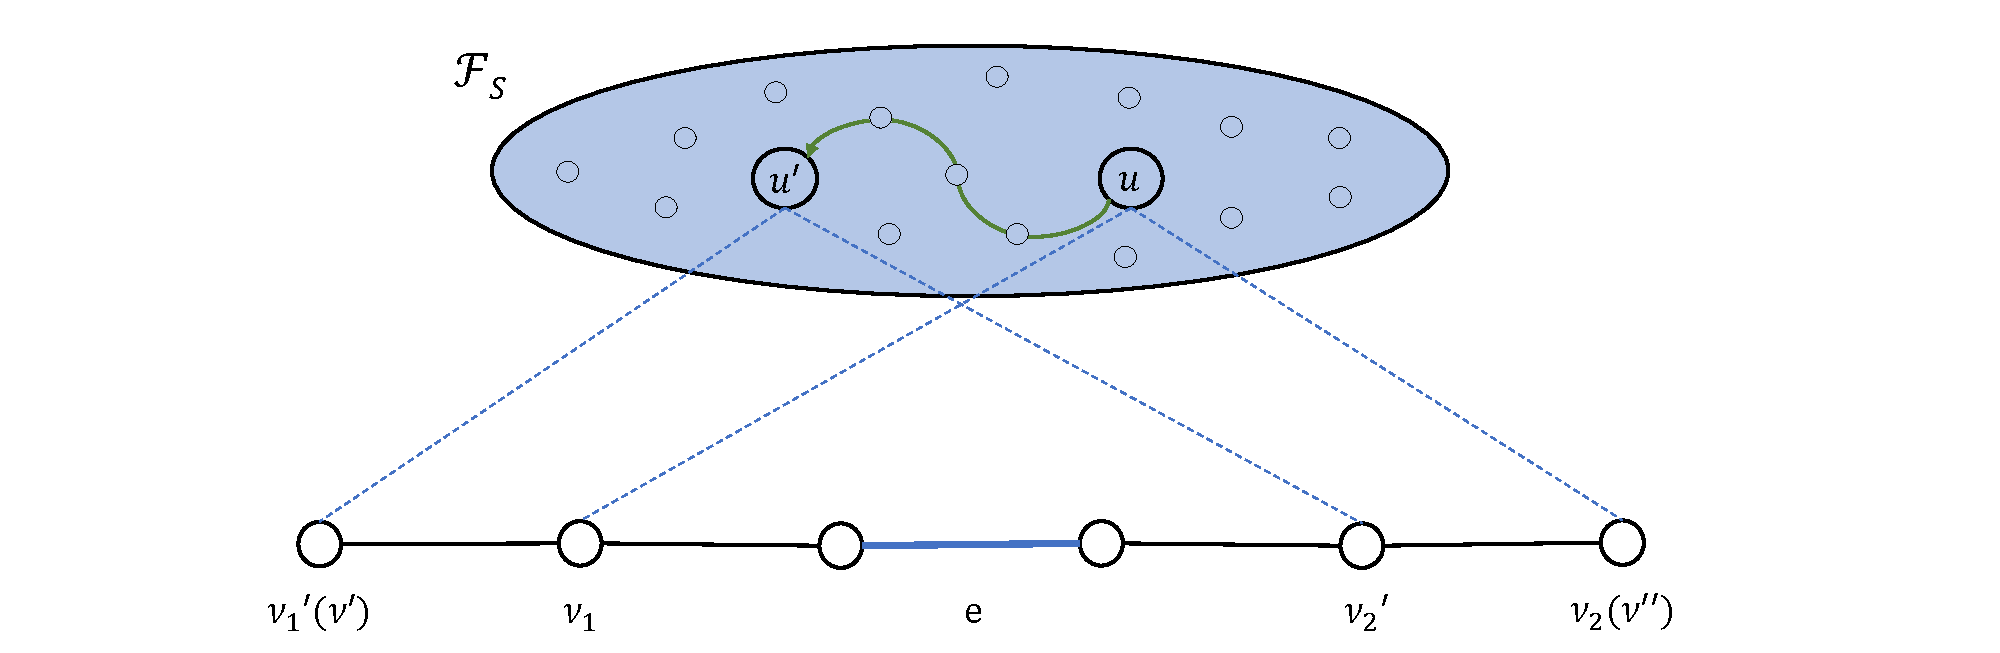
\includegraphics[width=0.95\textwidth]{src/images/proof-reachability-compressed.pdf}
    \caption{The structure of path $P(\nu',\nu'')$.}
\label{fig:structure-of-p(nu',nu'')}
\end{figure}

\end{proof}
% Lemma \ref{lem:contracted-subcactus-mincut} implies that vertex set compressed to each contracted node defines a Steiner mincut. This completes the proof of Lemma \ref{lem:u-u'-in-G-nu}.

Consider the set of non-terminals in the strip ${\cal D}_{s,t}$ that are not compressed to contracted vertex $v_c$. Let this set be $U$. Observe that the set of units $\bigcup_{u\in U} {\cal R}_s(u)$ form a Steiner mincut (using Lemma \ref{lem:reachability-cones}). Moreover, it follows from Lemma \ref{lem:u-u'-in-G-nu} that each non-terminal unit in the set $\bigcup_{u\in U} {\cal R}_s(u)$ is not compressed to contracted vertex $v_c$. Thus, $U = \bigcup_{u\in U} {\cal R}_s(u) \setminus \{\mathbf{s}\}$. All the set of vertices compressed to $v_c$ forms the complement of set $\bigcup_{u\in U} {\cal R}_s(u)$, and thus defines the same Steiner mincut. Therefore, the set of vertices corresponding to each contracted vertex defines a Steiner mincut.

It follows from the construction that $G_{S'}$ is a quotient graph of $G$. Moreover, the number of contracted vertices equals the number of cycles and tree edges incident on node $\nu$ in the skeleton.  We state the following lemma.




% $G_{S'}$ obtained after the $2-$step contraction procedure. 
% that will be required for answering the queries.

\begin{lemma}
Let $S'\subset S$ be a maximal subset of vertices such that $c_{S'}>c_S$ and $\nu$ be the node in ${\cal H}_S$ corresponding to $S'$. Let $G_{S'}$ be the graph obtained after %applying the above procedure.
$2$-step contraction procedure. 
\begin{enumerate}
    \item The set of vertices compressed to a contracted vertex defines a Steiner mincut for set $S$.
    \item The number of contracted vertices equals the number of cycles and tree edges incident on node $\nu$ in ${\cal H}_S$.
\end{enumerate}
\label{lem:contracted-subcactus-mincut}
\end{lemma}


\vspace{-8mm}
\section{Query transformation in \texorpdfstring{$G_{S'}$}{compact graph}}
% {\color{red} Motivation for this subsection is missing in the following start line.}

% The graph $G_{S'}$ does not even contain all edges of graph $G$ because a large portion of vertices is contracted. However, we can use the findings of Section \ref{sec:query-transformation} to effectively handle this problem. 
We begin with a lemma that was used by Gomory and Hu to build a tree storing all-pairs mincuts. 

\begin{lemma}[Gomory and Hu \cite{GH61}]
Let $A$ defines a $(s,t)$-mincut with $s\in A$. Let $r\in A$ be any vertex.
For any $(s,r)$-mincut, say defined by $B$, there exists a $(s,r)$-mincut that keeps $\bar A$ intact and still contains all edges in cut defined by $B$ that don't have both endpoints in $\bar A$.
\label{lem:GH}
\end{lemma}

Consider any two vertices $s,r\in S'$. Recall that $S'$ is mapped to $\nu$ in the skeleton ${\cal H}_S$. 
% Consider any cycle $c$ that passes through $\nu$ in the cactus. 
Let $A$ be the subset of vertices compressed to a contracted vertex in $G_{S'}$. Notice that all those $(s,r)$-mincuts in $G$ that keep $\bar{A}$ intact remain preserved in $G_{S'}$. Moreover, it follows from Lemma \ref{lem:contracted-subcactus-mincut} and Lemma \ref{lem:GH} that there is at least one such $(s,r)$-mincut. So it suffices to work with graph $G_{S'}$ if one wishes to calculate the value of $(s,r)$-mincut in $G$ or simply report a $(s,r)$-mincut in $G$
for any $s,r\in S$. Moreover, we can answer a query \textsc{edge-contained}$(s,r,E_y)$ using $G_{S'}$ if all edges in $E_y$ remain intact in graph $G_{S'}$. 
However, answering a query \textsc{edge-contained}$(s,r,E_{y})$ for any arbitrary $E_y$ using $G_{S'}$ is still challenging. This is because 
% we need to find at least one $(s,r)$-mincut in $G$ that contains all edges in $E_y$ but 
$G_{S'}$ may not even preserve all $(s,r)$-mincuts. In particular, all those $(s,r)$-mincuts that cut the set associated with a contracted vertex in $G_{S'}$ get lost during the transformation from $G$ to $G_{S'}$. We shall now establish a mapping from the set of all such lost $(s,r)$-mincuts to the set of $(s,r)$-mincuts that are present in $G_{S'}$. 

Let $y$ belong to $\bar{A}$. It follows from Lemma \ref{lem:contracted-subcactus-mincut} that the cut $(A,\bar{A})$ is a $(s,t)$-mincut for any $t\in S\cap \bar{A}$. Hence, $A,s,t,r$ satisfy all conditions of Theorem  \ref{thm:query-transform}. Now notice that entire $\bar{A}$
is compressed to a single vertex, say $y'$, in $G_{S'}$. Hence we can state the following Theorem.



\begin{theorem} \label{thm:edge-correspondence}
Given an undirected graph $G=(V,E)$, a subset $S\subseteq V$, let $S'\subset S$ be a maximal subset of vertices such that $c_{S'}>c_S$.
There exists a quotient graph $G_{S'}$ with the following property.~
For any two vertices $r,s \in S'$ and a set of edges $E_y$ incident on vertex $y$ in $G$, there exists a set of edges $E_{y'}$ incident on a vertex $y'$ in $G_{S'}$ such that $E_y$ lies in a $(r,s)$-mincut in $G$ if and only if $E_{y'}$ lies in a $(r,s)$-mincut in $G_{S'}$. 
\end{theorem}

We have already seen the construction of $G_{S'}$. In order to transform  \textsc{edge-contained}$(s,r,E_y)$ to \textsc{edge-contained}$(s,r,E_{y'})$  using Theorem \ref{thm:edge-correspondence}, we give an efficient algorithm for computing $E_{y'}$. Moreover, once we find a $(r,s)$-mincut in $G_{S'}$ that contains $E_{y'}$ we can efficiently compute a $(r,s)$-mincut in $G$ that contains all edges in $E_{y}$. Interestingly, we have algorithms that run in time linear in the size of flesh for both these tasks, stated in the following Lemma. 

\begin{lemma}
\label{lem:linear-time-qt}
Set of edges $E_{y'}$ in Theorem \ref{thm:edge-correspondence} can be obtained from $E_y$ given flesh ${\cal F}_S$ and skeleton $\mathcal H_S$ in time linear in the size of flesh.
\end{lemma}

\begin{lemma}
\label{lem:mincut-qt}
Given a $(r,s)$-mincut in $G_{S'}$ that contains the all edges in set $E_{y'}$, we can construct a $(r,s)$-mincut in $G$ that contains all edges in set $E_y$ in time linear in the size of flesh ${\cal F}_S$.
% (Proof follows from Corollary \ref{cor:query-transformation})
\end{lemma}

\begin{proof}
Consider the case when $y$ does not belong to any contracted vertex. In this case, all edges in $E_y$ remain intact in $G_{S'}$ and thus $E_{y'}=E_{y}$.

Now, suppose $y$ belong to contracted vertex $y'$. Let $\bar A$ be the set of vertices compressed to contracted vertex $y'$. We select a vertex $t\in {\bar A} \cap S$ and construct the ${\cal D}_{A,t}$ strip using the flesh ${\cal F}_S$ and skeleton ${\cal H}_S$ in time linear in the size of flesh (using Lemma \ref{lem:strip-from-carcass}). Using the construction outlined in Lemma \ref{lem:query-transformation} we can obtain the set of edges $E_{A}$ by computing reachability cone(s) in strip ${\cal D}_{A,t}$. This takes time linear in size of ${\cal D}_{A,t}$. All edges in $E_A$ share same endpoint $y'$ in $G_{S'}$. Thus, we get the set of edges $E_{y'}$ which is simply all edges in $G_{S'}$ corresponding to set $E_A$. Clearly, this process can be accomplished in time linear in the size of flesh ${\cal F}_S$.

Suppose we have a $(r,s)$-mincut in $G_{S'}$, say $B$ such that $s,t \not\in B$ that contains all edges in $E_{y'}$. If $y$ does not belong to any contracted vertex, this cut itself can be reported as $E_y=E_{y'}$. Suppose $y$ belong to contracted vertex $y'$. We can construct another $(r,s)$-mincut $B\cup R$ (recall the definition of $R$ in Proof of Lemma \ref{lem:query-transformation}). This procedure also involves construction of ${\cal D}_{A,t}$ strip and computation of reachability cone(s) in this strip. This process can also be accomplished in time linear in the size of flesh ${\cal F}_S$.
\end{proof}
\chapter{Compact Data Structures for Edge-Containment Queries}

We describe first a hierarchical data structure of Katz, Katz, Korman and Peleg \cite{DBLP:journals/siamcomp/KatzKKP04}
that was used for compact labeling scheme for all-pairs mincuts. This hierarchical data structure is actually a rooted tree, denoted by ${\cal T}_G$ henceforth. 
The key insight on which this tree is built is an equivalence relation defined for a Steiner set $S\subseteq V$ as follows.


\begin{definition}[Relation ${\cal R}_S$]
Any two vertices $a,b\in S$ are said to be related by ${\cal R}_S$, that is $(a,b)\in {\cal R}_S$, if
$c_{a,b}>c_S$, where $c_S$ is the value of a Steiner mincut of $S$.
\end{definition}

% \noindent
% The fact that ${\cal R}_S$ is an equivalence relation defined over $S$ can be easily derived using Lemma \ref{lem:triangle-inequality}.
% It can be observed that for any vertex $x\in S$, the equivalence class $[x]$ defined by ${\cal R}_S$ consists of all those vertices $y\in S$ such that the value of $(x,y)$-mincut is strictly greater than $c_S$. 


By using ${\cal R}_S$ for various carefully chosen instances of $S$, we can build the tree structure ${\cal T}_G$ in a top-down manner as follows. Each node $\nu$ of the tree will be associated with a Steiner set, denoted by $S(\nu)$, and the equivalence relation ${\cal R}_{S(\nu)}$. To begin with, for the root node $r$, we associate $S(r)=V$.
Using ${\cal  R}_{S(\nu)}$, we partition $S(\nu)$ into equivalence classes. For each equivalence class, we create a unique child node of $\nu$; the Steiner set associated with this child will be the corresponding equivalence class. We process the children of $\nu$ recursively along the same lines. We stop when the corresponding Steiner set is a single vertex. 

It follows from the construction described above that the tree ${\cal T}_G$ will have $n$ leaves - each corresponding to a vertex of $G$. The size of ${\cal T}_G$ will be $O(n)$ since each internal node has at least 2 children. Notice that $S(\nu)$ is the set of vertices present at the leaf nodes of the subtree of ${\cal T}_G$ rooted at $\nu$. The following observation captures the relationship between a parent and child node in 
${\cal T}_G$.

\begin{observation}
\label{obs:maximal-subset-subtree}
Suppose $\nu \in {\cal T}_G$ and $\mu$ is its parent. $S(\nu)$ comprises of a maximal subset of vertices in $S(\mu)$ with connectivity strictly greater than that of $S(\mu)$.
\end{observation}

The following observation conveys an important property about the value of $(s,t)$-mincut for any two vertices $s,t\in V$.

\begin{observation}
\label{obs:(s,t)-mincut-lca}
Suppose $s,t \in V$ are two vertices and $\mu$ is their LCA in ${\cal T}_G$ then $c_{s,t}=c_{S(\mu)}$.
\end{observation}



${\cal T}_G$ can be augmented to design a data structure for edge-containment query for any pair of vertices. For a single-edge-containment query, we get the following result.

\section{\texorpdfstring{An ${\cal O}(n^2)$}{A quadratic space} data structure for single edge-containment queries} \label{appendix:n2-ds}

% We build our ${\cal O}(n^2)$ data structure by augmenting each internal node $\nu$ of hierarchy tree ${\cal T}_G$ with the skeleton ${\cal H}_{S(\nu)}$ and projection mapping $\pi_{S(\nu)}$.

% Let $s,t$ be any two vertices such that $\nu$ is their LCA in ${\cal T}_G$. $s$ and $t$ must belong to different nodes in the the skeleton ${\cal H}_{S(\nu)}$ stored at $\nu$. Interestingly, the skeleton ${\cal H}_{S(\nu)}$ and the corresponding projection mapping $\pi_{S(\nu)}$ have sufficient information to infer whether any edge $(x,y)\in E$ belongs to some $(s,t)$-mincut. 
Suppose $S$ is a designated Steiner set and $s,t\in S$ are Steiner vertices separated by some Steiner mincut. We can determine if an edge $(x,y)\in E$ belongs to some $(s,t)$-mincut using the strip ${\cal D}_{s,t}$ that can be built from the connectivity carcass. However, the construction of strip requires ${\cal O}(\min(m,nc_S))$ time. Interestingly, we show that only the skeleton and the projection mapping of the connectivity carcass are sufficient for answering this query in constant time. Moreover, the skeleton and the projection mapping occupy only ${\cal O}(n)$ space compared to the ${\cal O}(\min(m,nc_S))$ space occupied by the entire connectivity carcass.


Similar to the projection mapping of the stretched units, Dinitz and Vainshtein \cite{DBLP:journals/siamcomp/DinitzV00} introduced the notion of projection mapping for edges as follows. Suppose $(x,y)\in E$. If $x$ and $y$ belong to the same unit, then $P(x,y) = \varnothing$. If $x$ and $y$ belong to distinct terminal units mapped to nodes, say $\nu_1$ and $\nu_2$, in the skeleton ${\cal H}_S$, then $P(x,y) = P(\nu_1,\nu_2)$. If at least one of them belongs to a stretched unit, $P(x,y)$ is the extended path defined in Lemma \ref{lem:path-extendable}. This allows us to state the following lemma which follows from the construction of a strip corresponding to a subbunch given in Section \ref{subsec:connectivity-carcass}.

\begin{lemma}[\cite{DBLP:conf/stoc/DinitzV94}]
Edge $(x,y)\in E$ appears in the strip corresponding to a subbunch if and only if one of the structural edge in the cut of ${\cal H}_S$ corresponding to this subbunch lies in $P(x,y)$.
\label{lem:edge-path-intersect-subbunch}
\end{lemma}

We state the necessary and sufficient condition for an edge $(x,y)$ to lie in an $(s,t)$-mincut. Note that two paths are said to intersect in the skeleton if the unique path of cycle and tree edges in both the paths intersect at some cycle or tree edge.
% The skeleton ${\cal H}_{S(\nu)}$ and the corresponding projection mapping $\pi_{S(\nu)}$ have the sufficient information to infer whether any edge $(x,y)\in E$ belongs to some $(s,t)$-mincut as stated by the following lemma. We say that two paths intersect if the unique path of cycle and tree edges in both the paths intersect at some cycle or tree edge.

\begin{lemma} \label{lem:path-intersects-tree}
 Edge $(x,y)\in E$ belongs to a $(s,t)$-mincut if and only if the proper path $P(x,y)$ intersects a path between the nodes containing $s$ and $t$ in in $\mathcal H_{S}$.
\end{lemma}
\begin{proof}
Observe that an edge $(x,y)$ lies in a $(s,t)$-mincut if and only if it appears in the strip ${\cal D}_{s,t}$ (follows from Lemma \ref{lem:E_y-edges-same-side}). Infact, we can extend this notion for subbunch as well. The edge $(x,y)$ lies in some $(s,t)$-mincut if and only if it appears in the strip corresponding to some subbunch that separates $s$ from $t$.

Consider each subbunch that separates $s$ from $t$. Let $\nu_1$ and $\nu_2$ be the nodes in ${\cal H}_S$ containing $s$ and $t$ respectively. A cut in ${\cal H}_S$ corresponding to any tree-edge (or pair of cycle edges in same cycle) in the path from $\nu_1$ to $\nu_2$ defines a subbunch separating $s$ from $t$. Moreover, it follows from the structure of the skeleton that no other cut in the skeleton corresponds to a subbunch separating $s$ from $t$. 

Suppose $(x,y)$ lies in some $(s,t)$-mincut. Thus, it must be in some subbunch separating $s$ from $t$. From the above discussion, we know that this subbunch must correspond to a cut in the path from $\nu_1$ to $\nu_2$ in skeleton ${\cal H}_S$. Moreover, it follows from Lemma \ref{lem:edge-path-intersect-subbunch} that $P(x,y)$ contains one of the structural edge in this cut. This implies that $P(x,y)$ intersects the path from $\nu_1$ to $\nu_2$ in skeleton ${\cal H}_S$.

Now, consider the other direction of this proof. Suppose $P(x,y)$ and the path from $\nu_1$ to $\nu_2$ intersect at some cycle (or tree edge) $c$. Let $e_1$ and $e_2$ be structural edges belonging to the cycle $c$ that are part of $P(x,y)$ and path from $\nu_1$ to $\nu_2$ respectively (in the case of tree edge $e_1=e_2=c$). Consider the cut in the skeleton corresponding to structural edges $e_1$ and $e_2$. It follows from Lemma \ref{lem:edge-path-intersect-subbunch} that $(x,y)$ lies in the strip corresponding to this subbunch. Since this cut separates $\nu_1$ from $\nu_2$ in ${\cal H}_S$, therefore the subbunch separates $s$ from $t$.
\end{proof}

We build our data structure using the findings of Lemma \ref{lem:path-intersects-tree}. We augment each internal node $\mu$ of the hierarchy tree ${\cal T}_G$ with the skeleton tree $T({\cal H}_{S(\mu)})$ and the projection mapping ${\pi}_{S(\mu)}$ corresponding to Steiner set $S(\mu)$. Since augmentation at each internal node takes ${\cal O}(n)$ space, therefore the total space occupied by the data structure is only ${\cal O}(n^2)$.


% Consider any node $\nu$ in ${\cal T}_G$.
% Let $s,t$ be any two vertices such that
% $\nu$ is their LCA in ${\cal T}_G$. $s$ and $t$ must belong to different nodes in the the skeleton ${\cal H}_{S(\nu)}$ stored at $\nu$. 
% It follows from Lemma \ref{lem:path-intersects-tree} that for a single-edge-containment query, we just have to keep the skeleton tree and the projection mapping at each internal node in ${\cal T}_G$. It is important to note that both these data structures collectively only take up ${\cal O}(n)$ space, contrary to the ${\cal O}(\min(m,nc_S)$ size taken up by the entire connectivity carcass. Thus, the size taken up by complete data structure is only ${\cal O}(n^2)$. 

Determining whether a given edge belongs to a $(s,t)$-mincut can be done as follows. Let $\mu$ be the LCA of $s$ and $t$ in ${\cal T}_G$. It follows from Observation \ref{obs:(s,t)-mincut-lca} that $c_{s,t}=c_{S(\mu)}$. Thus, $s$ and $t$ must be separated by some Steiner mincut for set $S(\mu)$. We check if paths $P(x,y)$ and $P(\pi_{S(\mu)}(s),\pi_{S(\mu)}(t))$ intersect in the skeleton ${\cal H}_{S(\mu)}$ (using Lemma \ref{lem:path-intersects-tree}). This can be done using ${\cal O}(1)$ LCA queries on the skeleton tree $T({\cal H}_{S(\mu)})$. Since it takes ${\cal O}(1)$ time for answering one LCA query \cite{DBLP:journals/jal/BenderFPSS05}, so the query time will be ${\cal O}(1)$ only. Algorithm \ref{algo:quadratic-space-query} presents a concise pseudocode of the query answering algorithm.

\begin{algorithm}%[H]
    \caption{Single edge-containment queries in ${\cal O}(n^2)$ data structure}
    \label{algo:quadratic-space-query}
    \begin{algorithmic}[1] % The number tells where the line numbering should start
        \Procedure{edge-cotained}{$s,t,x,y$}
            \State{${\mu}\gets$ LCA($\mathcal T_G,s,t$)}
            \State $\mathcal P_1 \gets P(\pi_{S(\mu)}(s),\pi_{S(\mu)}(t))$
            \State $\mathcal P_2 \gets P(x,y)$
            \If{$\mathcal P_1 \cap \mathcal P_2 = \varnothing$} 
            \State \textbf{return} False
            \Else 
            \State \textbf{ return} True
            \EndIf
        \EndProcedure
    \end{algorithmic}
\end{algorithm}
We can thus state the following theorem.
\begin{theorem}
 Given an undirected graph $G=(V,E)$ on $n=|V|$ vertices, there exists a data structure of 
${\cal O}(n^2)$ size that takes ${\cal O}(1)$ time to determine whether an edge $(x,y)\in E$
belongs to a $(s,t)$-mincut for any $s,t\in V$
and $(x,y)\in E$.
% \label{thm:O(n^2)-size-data-structure}
\end{theorem}

In the following section we present our ${\cal O}(m)$ size data structure which is more compact and can even handle multiple-edge-containment query.


\section{An \texorpdfstring{${\cal O}(m)$}{O(m)} size data structure for edge-containment queries}

Consider any node $\mu$ in ${\cal T}_G$. We associate a compact graph with node $\mu$, say $G_\mu=(V_\mu,E_\mu)$ with the following properties. 

\begin{enumerate}
    \item $G_\mu$ is a quotient graph of $G$ with $S(\mu)\subseteq V_\mu$
    \item  For each $s,t\in S(\mu)$ and a set of edges $E_y$ incident on vertex $y\in V$, there exists a set of edges $E_{y'}$ incident on vertex $y'\in V_\mu$ such that $E_y$ lies in a $(s,t)$-mincut in $G$ if and only if $E_{y'}$ lies in a $(s,t)$-mincut in $G_\mu$.
\end{enumerate}

For the root node $r$, $G_r=G$ and the two properties hold trivially.
We traverse ${\cal T}_G$ in a top down fashion to construct $G_\mu$ for each node $\mu \in {\cal T}_G$ as follows. Let $\mu$ be the parent of $\mu'$ in ${\cal T}_G$. Assume we have graph $G_{\mu}$ already built with the properties mentioned above. Thus, $S(\mu)\subseteq V_\mu$. Using Observation \ref{obs:maximal-subset-subtree} we know that $S(\mu')$ is a maximal subset of $S(\mu)$ with connectivity strictly greater than that of $S(\mu)$. Using Theorem \ref{thm:edge-correspondence} with $S=S(\mu)$ and $S'=S(\mu')$, it can be shown that there exists a graph $G_{S(\mu')}$ 
% such that -- for each $s,t \in S(\nu)$ and set of edges $E_y$ incident on vertex $y\in V_{\mu}$ there exists a set of edges $E_{y'}$ incident on vertex $y'\in V_\nu$ such that $E_y$ lies in a $(s,t)$-mincut in $G_\mu$ if and only if $E_{y'}$ lies in a $(s,t)$-mincut in $G_\nu$. This also implies that the above $2$ properties will hold for $G_\nu$.
that satisfies both the properties above. We define $G_{\mu'}$ to be $G_{S(\mu')}$.
The graph $G_{\mu'}$ itself
can be obtained using the $2$-step contraction procedure described in Section \ref{sec:compact-graph}.


% We use Property 1 and Observation \ref{obs:maximal-subset-subtree} to build the graph $G_\nu$ for the subset $S(\nu)$ from $G_\mu$ following the procedure described in Section \ref{sec:compact-graph}. Using Theorem \ref{thm:edge-correspondence}, it follows that $G_\nu$ also satisfies Property 2.

Our compact data structure will be ${\cal T}_G$ where each node $\mu$ will be augmented with the connectivity carcass of $S(\mu)$ in graph $G_\mu$. 

\subsection{The query algorithm}

A query \textsc{edge-contained}$(s,t,E_y)$ can be answered by the data structure as follows. We start from the root node of ${\cal T}_G$ and traverse the path to the node $\nu$ which is the LCA of $s$ and $t$. Consider any edge $(\mu,\mu')$ on this path, where $\mu$ is parent of $\mu'$. We modify the query \textsc{edge-contained}$(s,t,E_y)$ in $G_{\mu}$ to an equivalent query \textsc{edge-contained}$(s,t,E_{y'})$ in $G_{\mu'}$ as we move to $\mu'$ (see Theorem \ref{thm:edge-correspondence}). This computation can be carried out in time linear in size of flesh at node $\mu$ using Lemma \ref{lem:linear-time-qt}. We stop when $\mu = \nu$. Observe that $c_{s,t} = c_{S(\nu)}$ (using Observation \ref{obs:(s,t)-mincut-lca}) and thus must be separated by some Steiner mincut for $S(\nu)$.
Thus we compute the strip ${\cal D}_{s,t}$ at node $\nu$ and answer the edge-containment query using Lemma \ref{lem:E_y-edges-same-side}. If the query evaluates to true, we compute a $(s,t)$-mincut in $G_\nu$ using ${\cal D}_{s,t}$ that contains the required set of edges at this level. We retrace the path from $\nu$ to the root of ${\cal T}_G$.
% A $(s,t)$-mincut containing the edges in $E_y$ can be obtained as follows. We start from the LCA of $s$ and $t$ in ${\cal T}_G$, say $\nu$. We construct the strip ${\cal D}_{s,t}$ and obtain a $(s,t)$-mincut that contains the required set of edges. We traverse the path from $\nu$ to the root of ${\cal T}_G$.
Consider any edge $(\mu,\mu')$ on this path where $\mu$ is parent of $\mu'$. We find a corresponding $(s,t)$-mincut in graph $G_\mu$ from the $(s,t)$-mincut of $G_{\mu'}$ using Lemma \ref{lem:mincut-qt}. We stop at the root node and report the set of vertices defining the $(s,t)$-mincut in $G$.
We can thus state the following theorem.

\begin{theorem}
Given an undirected graph $G=(V,E)$ on $n=|V|$ vertices and $m=|E|$ edges, there exists a data structure of ${\cal O}(m)$ size that can determine whether any given subset of edges $E_y$ incident on vertex $y$ belongs to a $(s,t)$-mincut for any $s,t,y\in V$ and report the same if exists. The time taken to answer this query is ${\cal O}(\min(m,nc_{s,t}))$.
\label{thm:O(m)-size-data-structure}
\end{theorem}

\subsection{Size and Time analysis of compact data structure}
\label{appendix:size-time-analysis-compact-ds}

The data structure doesn't seem to be an ${\cal O}(m)$ size data structure at first sight. Observe that augmentation at any internal node can still take ${\cal O}(m)$ space individually. Interestingly, we show that collective space taken by augmentation at each internal node will still be ${\cal O}(m)$.

We begin with the following lemma which gives a tight bound on the sum of weights of edges in Gomory-Hu tree is $\Theta(m)$. We also give the proof for the same which was suggested in \cite{DBLP:conf/stoc/HariharanKPB07,DBLP:journals/siamcomp/DinitzV00}.

\begin{lemma}[\cite{DBLP:conf/stoc/HariharanKPB07,DBLP:journals/siamcomp/DinitzV00}]
\label{fact:GH-weight}
The sum of weights of all edges in the Gomory-Hu tree is ${\Theta}(m)$.
\end{lemma}
\begin{proof}
Consider any edge $(u,v)\in E$. This edge must be present in every $(u,v)$-mincut. Thus, the sum of weights of all edges in Gomory-Hu tree is at least $m$. Now, root the Gomory-Hu tree at any arbitrary vertex $r$. Let $f$ maps each edge in this tree to its lower end-point. It is easy to observe that $f$ is a one-to-one mapping. Let $e$ be an edge in the Gomory-Hu tree. Observe that $w(e) \leq deg(f(e))$ (where $deg()$ is the degree of vertex in $G$). Thus the sum of weights of all edges in Gomory-Hu tree is at most $2m$. This comes from the simple observation that the sum of the degree of all vertices in $G$ equals $2m$.
\end{proof}

Let us assign each edge $(\mu,\mu')$ in the hierarchy tree ${\cal T}_G$ weight equal to the Steiner mincut value for the Steiner set $S(\mu)$ (if $\mu$ is the parent of $\mu'$). We shall show that sum of the weight of edges in hierarchy tree ${\cal T}_G$ is $\Theta(m)$. %This will help in our analysis later.

To establish this bound refer to algorithm \ref{Construct Tree} that gives an algorithm to construct the hierarchy tree from Gomory-Hu tree. Observe that the variable $ctr$ in this algorithm stores the sum of weights of all edges in ${\cal T}_G$. It is clear that for $k$ edges removed from the Gomory-Hu tree, we add $k+1$ edges of equal weight in ${\cal T}_G$. Thus, the sum of the weight of all edges in ${\cal T}_G$ is at most $4m$ (since $k+1 \leq 2k$). Therefore, we state the following lemma.

\begin{algorithm}%[H]
    \caption{Construct Hierarchy Tree ${\cal T}_G$ from Gomory-Hu Tree $\hat{ \cal T}_{G}$}
    \label{Construct Tree}
    \begin{algorithmic}[1] % The number tells where the line numbering should start
        \State $ctr \gets 0$
        \Procedure{Construct-Tree}{$\hat{ \cal T}_{G}$}
            \If{$\hat{ \cal T}_{G}$ has single node}
            \State Create a node $\mu$
            \State $val(\mu) \gets val(\hat{ \cal T}_{G})$
            \State \textbf{return} $\mu$
            \EndIf
            \State $c_{\min} \gets$ $\min_{e\in \hat{ \cal T}_{G}}w(e)$
            \State Let there be $k$ edges with weight $c_{\min}$
            \State Remove all edges of weight $c_{\min}$ in $\hat{ \cal T}_{G}$ to get $(k+1)$ trees $T_1,..,T_{k+1}$
            \State Create a node $\mu$
            \State $ctr \gets ctr + c_{\min}\times(k+1)$
            \State $children(\mu) \gets \{\textsc{Construct-Tree}(T_i)\;|\;\forall i\in [k+1]\}$
            \State \textbf{return} $\mu$
        \EndProcedure
    \end{algorithmic}
\end{algorithm}

\begin{lemma}
\label{lem:hierarchy-tree-weight}
The sum of weights of all edges in the tree ${\cal T}_G$ is ${\Theta}(m)$.
\end{lemma}
% The size and time analysis of the data structure crucially exploits the following observations,
We shall now give a bound on the size of connectivity carcass augmented at each internal node. The following lemma gives a bound on the size of flesh graph ${\cal F}_S$ for any Steiner set $S$.

\begin{lemma}
Let ${\cal V}_S$ and ${\cal W}_S$ denote the set of Steiner and non-Steiner units respectively in flesh graph ${\cal F}_S$ with Steiner set $S\subseteq V$. The size of ${\cal F}_S$ is bounded by $|{\cal V}_S|c_S + \sum_{u\in {\cal W}_S}deg(u)$.
\label{lem:size-of-flesh}
\end{lemma}
\begin{proof}
Consider the Gomory-Hu tree of the flesh ${\cal F}_S$, say ${\cal T}$. It is evident that the value of mincut between any two units is at most $c_S$. This follows from the definition of a unit. Now, root this tree ${\cal T}$ at some Steiner unit. Let $f$ maps each edge in this tree to its lower end-point. Any edge in this tree has weight at most $c_S$. However, for any non-Steiner unit $u$, $w(f^{-1}(u)) \leq deg(u)$ (where $deg()$ is the degree of vertex in $G$).  Thus, the sum of weight of all edges in ${\cal T}$ is bounded by $|{\cal V}_S|c_S + \sum_{u\in {\cal W}_S}deg(u)$. Using Lemma \ref{fact:GH-weight}, it follows that size of flesh ${\cal F}_S$ is bounded by $|{\cal V}_S|c_S + \sum_{u\in {\cal W}_S}deg(u)$.
\end{proof}

Consider the flesh graph ${\cal F}_{S(\mu)}$ stored at some internal node $\mu$ in the tree. Let ${\cal V}_{S(\mu)}$ and ${\cal W}_{S(\mu)}$ denote the set of Steiner and non-Steiner units respectively in ${\cal F}_{S(\mu)}$. Let $u$ be some non-Steiner unit in ${\cal F}_{S(\mu)}$. It is evident that $u$ consists of only contracted vertices (obtained after the contraction procedure at some ancestral node). This non-Steiner unit gets compressed to a new contracted vertex in all descendants, and in a sense, disappears. Thus, each contracted vertex appears in at most one non-Steiner unit. 

Now, we shall count the total number of contracted vertices introduced at each internal node. We know that this count is an upper bound on the total number of non-Steiner units across all flesh graphs. It follows from Lemma \ref{lem:contracted-subcactus-mincut} that the number of contracted vertices introduced by node $\mu$ to the graph $G_{\mu'}$ associated with its child $\mu'$ is equal to the number of cycles and tree edges incident on node corresponding to $\mu'$ in skeleton ${\cal H}_{S(\mu)}$. We sum this number for each child of $\mu$. The total number of contracted vertices introduced by internal node $\mu$ to all its children is at most twice the number of tree and cycle edges. Since the skeleton is a cactus graph, thus the number of tree and cycle edges is ${\cal O}(|{\cal V}_{S(\mu)}|)$. Moreover, we know that the number of Steiner units in ${\cal F}_{S(\mu)}$ also equals the number of children of node $\mu$ in tree ${\cal T}_G$. Therefore, the number of Steiner units across all flesh graphs stored at each internal node is given by ${\sum}_{\mu \in {\cal T}_G}|{\cal V}_{S(\mu)}|$ which is ${\cal O}(n)$. Thus, the total number of non-Steiner units across all flesh graphs is also ${\cal O}(n)$.

Now, we shall bound the sum of the degree of all non-Steiner units across all flesh graphs. Since each contracted vertex appears in at most one non-Steiner unit, we can sum the degree of all contracted vertices to get an upper bound. It again follows from Lemma \ref{lem:contracted-subcactus-mincut} that the degree of contracted vertex introduced by node $\mu$ is exactly $c_{S(\mu)}$. Thus, the sum of degree of all contracted vertices introduced by node $\mu$ is ${\cal O}(|{\cal V}_{S(\mu)}|c_{S(\mu)})$.

Combining the above observations, we can infer the following.


\begin{inference}
\label{inf:units-O(n)}
The total number of units across all flesh graphs is ${\cal O}(n)$.
\end{inference}
\begin{inference}
\label{inf:sum-degree}
The sum of degree of non-Steiner units across all flesh graphs stored at each internal node $\mu$ is ${\cal O}(\sum_{\mu \in {\cal T}_G}{|{\cal V}_{S(\mu)}|}c_{S(\mu)})$ i.e ${\cal O}(m)$ (follows from Lemma \ref{lem:hierarchy-tree-weight}). In other words, $\sum_{\mu \in {\cal T}_G} \sum_{u \in {\cal W}_{S(\mu)}}deg(u)$ is ${\cal O}(m)$.
\end{inference}


\subsubsection*{Size analysis of Data Structure}
Combining Lemma \ref{fact:GH-weight}, Lemma \ref{lem:hierarchy-tree-weight}, Lemma \ref{lem:size-of-flesh} and Inference \ref{inf:sum-degree} we get the following result.
\begin{equation*}
    \begin{split}
        \nonumber
        \sum_{\mu \in {\cal T}_G}|{\cal F}_{S(\mu)}| &\leq c_1 \times \sum_{\mu \in {\cal T}_G} (|{\cal V}_{S(\mu)}|c_{S(\mu)} + \sum_{u\in {\cal W}_{S(\mu)}}deg(u))\\
        &\leq c_2 \times m
    \end{split}
\end{equation*}


\subsubsection*{Time analysis of Data Structure}

A trivial bound on the query time follows from the size analysis itself. Since the combined size of our data structure is ${\cal O}(m)$, it follows that the sum of sizes of all flesh graphs from the root node to $LCA(s,t)$ will also be ${\cal O}(m)$. Dinitz and Vainshtein \cite{DBLP:conf/stoc/DinitzV94} showed that size of flesh graph ${\cal F}_S$ is ${\cal O}(\tilde{n}c_S)$ for Steiner set $S$, where $\tilde{n}$ is the number of units in the flesh graph. Total number of units across all flesh graphs is only ${\cal O}(n)$ (Inference \ref{inf:units-O(n)}). The value of Steiner mincut increases as we traverse from the root towards a leaf. Thus, $c_{s,t}$ is the maximum Steiner mincut value in the path from root node to $LCA(s,t)$ . Thus, the sum of sizes of all flesh graphs in this path is bounded by ${\cal O}(nc_{s,t})$. Thus, the query time we achieve is ${\cal O}(\min(m,nc_{s,t}))$.
%% This defines the bibliography file (main.bib) and the bibliography style.
%% If you want to create a bibliography file by hand, change the contents of
%% this file to a `thebibliography' environment.  For more information 
%% see section 4.3 of the LaTeX manual.
% \begin{singlespace}
\bibliography{main}
\bibliographystyle{plain}
% \end{singlespace}

\end{document}

